\documentclass[twoside]{book}

% Packages required by doxygen
\usepackage{fixltx2e}
\usepackage{calc}
\usepackage{doxygen}
\usepackage[export]{adjustbox} % also loads graphicx
\usepackage{graphicx}
\usepackage[utf8]{inputenc}
\usepackage{makeidx}
\usepackage{multicol}
\usepackage{multirow}
\PassOptionsToPackage{warn}{textcomp}
\usepackage{textcomp}
\usepackage[nointegrals]{wasysym}
\usepackage[table]{xcolor}

% Font selection
\usepackage[T1]{fontenc}
\usepackage[scaled=.90]{helvet}
\usepackage{courier}
\usepackage{amssymb}
\usepackage{sectsty}
\renewcommand{\familydefault}{\sfdefault}
\allsectionsfont{%
  \fontseries{bc}\selectfont%
  \color{darkgray}%
}
\renewcommand{\DoxyLabelFont}{%
  \fontseries{bc}\selectfont%
  \color{darkgray}%
}
\newcommand{\+}{\discretionary{\mbox{\scriptsize$\hookleftarrow$}}{}{}}

% Page & text layout
\usepackage{geometry}
\geometry{%
  a4paper,%
  top=2.5cm,%
  bottom=2.5cm,%
  left=2.5cm,%
  right=2.5cm%
}
\tolerance=750
\hfuzz=15pt
\hbadness=750
\setlength{\emergencystretch}{15pt}
\setlength{\parindent}{0cm}
\setlength{\parskip}{3ex plus 2ex minus 2ex}
\makeatletter
\renewcommand{\paragraph}{%
  \@startsection{paragraph}{4}{0ex}{-1.0ex}{1.0ex}{%
    \normalfont\normalsize\bfseries\SS@parafont%
  }%
}
\renewcommand{\subparagraph}{%
  \@startsection{subparagraph}{5}{0ex}{-1.0ex}{1.0ex}{%
    \normalfont\normalsize\bfseries\SS@subparafont%
  }%
}
\makeatother

% Headers & footers
\usepackage{fancyhdr}
\pagestyle{fancyplain}
\fancyhead[LE]{\fancyplain{}{\bfseries\thepage}}
\fancyhead[CE]{\fancyplain{}{}}
\fancyhead[RE]{\fancyplain{}{\bfseries\leftmark}}
\fancyhead[LO]{\fancyplain{}{\bfseries\rightmark}}
\fancyhead[CO]{\fancyplain{}{}}
\fancyhead[RO]{\fancyplain{}{\bfseries\thepage}}
\fancyfoot[LE]{\fancyplain{}{}}
\fancyfoot[CE]{\fancyplain{}{}}
\fancyfoot[RE]{\fancyplain{}{\bfseries\scriptsize Generated by Doxygen }}
\fancyfoot[LO]{\fancyplain{}{\bfseries\scriptsize Generated by Doxygen }}
\fancyfoot[CO]{\fancyplain{}{}}
\fancyfoot[RO]{\fancyplain{}{}}
\renewcommand{\footrulewidth}{0.4pt}
\renewcommand{\chaptermark}[1]{%
  \markboth{#1}{}%
}
\renewcommand{\sectionmark}[1]{%
  \markright{\thesection\ #1}%
}

% Indices & bibliography
\usepackage{natbib}
\usepackage[titles]{tocloft}
\setcounter{tocdepth}{3}
\setcounter{secnumdepth}{5}
\makeindex

% Hyperlinks (required, but should be loaded last)
\usepackage{ifpdf}
\ifpdf
  \usepackage[pdftex,pagebackref=true]{hyperref}
\else
  \usepackage[ps2pdf,pagebackref=true]{hyperref}
\fi
\hypersetup{%
  colorlinks=true,%
  linkcolor=blue,%
  citecolor=blue,%
  unicode%
}

% Custom commands
\newcommand{\clearemptydoublepage}{%
  \newpage{\pagestyle{empty}\cleardoublepage}%
}

\usepackage{caption}
\captionsetup{labelsep=space,justification=centering,font={bf},singlelinecheck=off,skip=4pt,position=top}

%===== C O N T E N T S =====

\begin{document}

% Titlepage & ToC
\hypersetup{pageanchor=false,
             bookmarksnumbered=true,
             pdfencoding=unicode
            }
\pagenumbering{alph}
\begin{titlepage}
\vspace*{7cm}
\begin{center}%
{\Large Galactic Clash }\\
\vspace*{1cm}
{\large Generated by Doxygen 1.8.14}\\
\end{center}
\end{titlepage}
\clearemptydoublepage
\pagenumbering{roman}
\tableofcontents
\clearemptydoublepage
\pagenumbering{arabic}
\hypersetup{pageanchor=true}

%--- Begin generated contents ---
\chapter{Hierarchical Index}
\section{Class Hierarchy}
This inheritance list is sorted roughly, but not completely, alphabetically\+:\begin{DoxyCompactList}
\item \contentsline{section}{B\+DD}{\pageref{class_b_d_d}}{}
\item \contentsline{section}{Bordure}{\pageref{class_bordure}}{}
\item \contentsline{section}{enregistrement\+B\+DD}{\pageref{classenregistrement_b_d_d}}{}
\item \contentsline{section}{Entite}{\pageref{class_entite}}{}
\begin{DoxyCompactList}
\item \contentsline{section}{Ennemi}{\pageref{class_ennemi}}{}
\begin{DoxyCompactList}
\item \contentsline{section}{Ennemi1}{\pageref{class_ennemi1}}{}
\item \contentsline{section}{Ennemi2}{\pageref{class_ennemi2}}{}
\item \contentsline{section}{Ennemi3}{\pageref{class_ennemi3}}{}
\item \contentsline{section}{Ennemi\+Boss}{\pageref{class_ennemi_boss}}{}
\item \contentsline{section}{Missile\+Ennemi}{\pageref{class_missile_ennemi}}{}
\end{DoxyCompactList}
\item \contentsline{section}{Etoiles}{\pageref{class_etoiles}}{}
\item \contentsline{section}{Joueur}{\pageref{class_joueur}}{}
\item \contentsline{section}{Missile}{\pageref{class_missile}}{}
\end{DoxyCompactList}
\item \contentsline{section}{Explosion}{\pageref{class_explosion}}{}
\item \contentsline{section}{Game}{\pageref{class_game}}{}
\item \contentsline{section}{High\+Score}{\pageref{class_high_score}}{}
\item \contentsline{section}{Niveaux}{\pageref{class_niveaux}}{}
\item \contentsline{section}{Texte}{\pageref{class_texte}}{}
\end{DoxyCompactList}

\chapter{Class Index}
\section{Class List}
Here are the classes, structs, unions and interfaces with brief descriptions\+:\begin{DoxyCompactList}
\item\contentsline{section}{\mbox{\hyperlink{class_b_d_d}{B\+DD}} \\*Classe g�rant la cr�ation de la \mbox{\hyperlink{class_b_d_d}{B\+DD}} }{\pageref{class_b_d_d}}{}
\item\contentsline{section}{\mbox{\hyperlink{class_bordure}{Bordure}} \\*Classe permettant de g�rer les bordures de l\textquotesingle{}�cran }{\pageref{class_bordure}}{}
\item\contentsline{section}{\mbox{\hyperlink{class_ennemi}{Ennemi}} \\*Classe de cr�ation des vaisseaux ennemis }{\pageref{class_ennemi}}{}
\item\contentsline{section}{\mbox{\hyperlink{class_ennemi1}{Ennemi1}} }{\pageref{class_ennemi1}}{}
\item\contentsline{section}{\mbox{\hyperlink{class_ennemi2}{Ennemi2}} }{\pageref{class_ennemi2}}{}
\item\contentsline{section}{\mbox{\hyperlink{class_ennemi3}{Ennemi3}} }{\pageref{class_ennemi3}}{}
\item\contentsline{section}{\mbox{\hyperlink{class_ennemi_boss}{Ennemi\+Boss}} }{\pageref{class_ennemi_boss}}{}
\item\contentsline{section}{\mbox{\hyperlink{classenregistrement_b_d_d}{enregistrement\+B\+DD}} \\*Cette classe permet de cr�er un objet qui facilite la r�cup�ration des donn�es dans la \mbox{\hyperlink{class_b_d_d}{B\+DD}} }{\pageref{classenregistrement_b_d_d}}{}
\item\contentsline{section}{\mbox{\hyperlink{class_entite}{Entite}} \\*Cette classe est la base de la plupart des objets cr��s dans le jeu. Elle poss�de un sprite et une forme }{\pageref{class_entite}}{}
\item\contentsline{section}{\mbox{\hyperlink{class_etoiles}{Etoiles}} \\*Permet la cr�ation des �toiles pour le background }{\pageref{class_etoiles}}{}
\item\contentsline{section}{\mbox{\hyperlink{class_explosion}{Explosion}} \\*Gestion des explosions du joueur et de la m�ga bombe }{\pageref{class_explosion}}{}
\item\contentsline{section}{\mbox{\hyperlink{class_game}{Game}} \\*Cette classe g�re la logique des �vennements du jeu et l\textquotesingle{}affichage }{\pageref{class_game}}{}
\item\contentsline{section}{\mbox{\hyperlink{class_high_score}{High\+Score}} \\*Cr�ation de la table de score }{\pageref{class_high_score}}{}
\item\contentsline{section}{\mbox{\hyperlink{class_joueur}{Joueur}} \\*Classe de cr�ation du joueur }{\pageref{class_joueur}}{}
\item\contentsline{section}{\mbox{\hyperlink{class_missile}{Missile}} \\*Projectiles du joueur (2 types, missile et canon) }{\pageref{class_missile}}{}
\item\contentsline{section}{\mbox{\hyperlink{class_missile_ennemi}{Missile\+Ennemi}} \\*Classe de cr�ation des projectiles des ennemis }{\pageref{class_missile_ennemi}}{}
\item\contentsline{section}{\mbox{\hyperlink{class_niveaux}{Niveaux}} \\*Classe de cr�ation des niveaux faisant office d\textquotesingle{}�diteur de niveaux }{\pageref{class_niveaux}}{}
\item\contentsline{section}{\mbox{\hyperlink{class_texte}{Texte}} \\*Classe de cr�ation des texte S\+F\+ML � afficher � l\textquotesingle{}�cran }{\pageref{class_texte}}{}
\end{DoxyCompactList}

\chapter{Class Documentation}
\hypertarget{class_b_d_d}{}\section{B\+DD Class Reference}
\label{class_b_d_d}\index{B\+DD@{B\+DD}}


Classe g�rant la cr�ation de la \mbox{\hyperlink{class_b_d_d}{B\+DD}}.  




{\ttfamily \#include $<$B\+D\+D.\+h$>$}

\subsection*{Public Member Functions}
\begin{DoxyCompactItemize}
\item 
\mbox{\Hypertarget{class_b_d_d_ac496884b98cc0a57192b7b507f5dc38c}\label{class_b_d_d_ac496884b98cc0a57192b7b507f5dc38c}} 
void {\bfseries open\+Database} ()
\item 
\mbox{\Hypertarget{class_b_d_d_a147be90295ed937f3d450f0c3aeeb3ee}\label{class_b_d_d_a147be90295ed937f3d450f0c3aeeb3ee}} 
void \mbox{\hyperlink{class_b_d_d_a147be90295ed937f3d450f0c3aeeb3ee}{close\+Database}} ()
\begin{DoxyCompactList}\small\item\em Fonction d\textquotesingle{}ouverture de la base de donn�es. \end{DoxyCompactList}\item 
\mbox{\Hypertarget{class_b_d_d_a739300647fc688e854aec5dc2aaa606b}\label{class_b_d_d_a739300647fc688e854aec5dc2aaa606b}} 
bool \mbox{\hyperlink{class_b_d_d_a739300647fc688e854aec5dc2aaa606b}{execute\+Query}} (std\+::string query)
\begin{DoxyCompactList}\small\item\em Fonction de fermeture de la base de donn�es. \end{DoxyCompactList}\item 
\mbox{\Hypertarget{class_b_d_d_a8031fec345574ff44abe2491b75b0073}\label{class_b_d_d_a8031fec345574ff44abe2491b75b0073}} 
bool {\bfseries insert\+Score} (std\+::string nom, int score)
\item 
\mbox{\Hypertarget{class_b_d_d_a9c14215b42c02cfdfb6774a28f7517a1}\label{class_b_d_d_a9c14215b42c02cfdfb6774a28f7517a1}} 
std\+::vector$<$ \mbox{\hyperlink{classenregistrement_b_d_d}{enregistrement\+B\+DD}} $\ast$ $>$ $\ast$ \mbox{\hyperlink{class_b_d_d_a9c14215b42c02cfdfb6774a28f7517a1}{get\+High\+Score}} ()
\begin{DoxyCompactList}\small\item\em Fonction permettant d\textquotesingle{}�crire dans la \mbox{\hyperlink{class_b_d_d}{B\+DD}}. \end{DoxyCompactList}\end{DoxyCompactItemize}
\subsection*{Public Attributes}
\begin{DoxyCompactItemize}
\item 
\mbox{\Hypertarget{class_b_d_d_addcb41f87c2c17d3cde49aea698158db}\label{class_b_d_d_addcb41f87c2c17d3cde49aea698158db}} 
std\+::string \mbox{\hyperlink{class_b_d_d_addcb41f87c2c17d3cde49aea698158db}{dbfile}}
\begin{DoxyCompactList}\small\item\em R�cup�ration des 6 meilleurs scores. \end{DoxyCompactList}\item 
\mbox{\Hypertarget{class_b_d_d_a86db71551298c29c84cfbbe45e16b368}\label{class_b_d_d_a86db71551298c29c84cfbbe45e16b368}} 
sqlite3 $\ast$ \mbox{\hyperlink{class_b_d_d_a86db71551298c29c84cfbbe45e16b368}{db}}
\begin{DoxyCompactList}\small\item\em Chemin d\textquotesingle{}acc�s de la \mbox{\hyperlink{class_b_d_d}{B\+DD}}. \end{DoxyCompactList}\end{DoxyCompactItemize}


\subsection{Detailed Description}
Classe g�rant la cr�ation de la \mbox{\hyperlink{class_b_d_d}{B\+DD}}. 

The documentation for this class was generated from the following files\+:\begin{DoxyCompactItemize}
\item 
prog/B\+D\+D.\+h\item 
prog/B\+D\+D.\+cpp\end{DoxyCompactItemize}

\hypertarget{class_bordure}{}\section{Bordure Class Reference}
\label{class_bordure}\index{Bordure@{Bordure}}


Classe permettant de g�rer les bordures de l\textquotesingle{}�cran.  




{\ttfamily \#include $<$Bordure.\+h$>$}

\subsection*{Public Member Functions}
\begin{DoxyCompactItemize}
\item 
\mbox{\Hypertarget{class_bordure_ab8b140bc1cb7b30e2acb602565b5ee2d}\label{class_bordure_ab8b140bc1cb7b30e2acb602565b5ee2d}} 
{\bfseries Bordure} (sf\+::\+Vector2f position, sf\+::\+Vector2f \mbox{\hyperlink{class_bordure_a04826325b0eced5ff5a808da13930b33}{taille}})
\item 
\mbox{\Hypertarget{class_bordure_af1067a674320ade211b01b5022b336db}\label{class_bordure_af1067a674320ade211b01b5022b336db}} 
void {\bfseries contruire} (sf\+::\+Render\+Window \&window)
\end{DoxyCompactItemize}
\subsection*{Public Attributes}
\begin{DoxyCompactItemize}
\item 
\mbox{\Hypertarget{class_bordure_aeaca331c70acff61056f986536bbcea9}\label{class_bordure_aeaca331c70acff61056f986536bbcea9}} 
sf\+::\+Rectangle\+Shape \mbox{\hyperlink{class_bordure_aeaca331c70acff61056f986536bbcea9}{forme}}
\begin{DoxyCompactList}\small\item\em Fonction permettant de \char`\"{}construire\char`\"{} (donc de mat�rialiser) les bordures invisible de l\textquotesingle{}�cran. \end{DoxyCompactList}\item 
\mbox{\Hypertarget{class_bordure_a04826325b0eced5ff5a808da13930b33}\label{class_bordure_a04826325b0eced5ff5a808da13930b33}} 
sf\+::\+Vector2f \mbox{\hyperlink{class_bordure_a04826325b0eced5ff5a808da13930b33}{taille}}
\begin{DoxyCompactList}\small\item\em forme repr�sentant la bordure \end{DoxyCompactList}\end{DoxyCompactItemize}


\subsection{Detailed Description}
Classe permettant de g�rer les bordures de l\textquotesingle{}�cran. 

The documentation for this class was generated from the following files\+:\begin{DoxyCompactItemize}
\item 
prog/Bordure.\+h\item 
prog/Bordure.\+cpp\end{DoxyCompactItemize}

\hypertarget{class_ennemi}{}\section{Ennemi Class Reference}
\label{class_ennemi}\index{Ennemi@{Ennemi}}


Classe de cr�ation des vaisseaux ennemis.  




{\ttfamily \#include $<$Ennemi.\+h$>$}

Inheritance diagram for Ennemi\+:\begin{figure}[H]
\begin{center}
\leavevmode
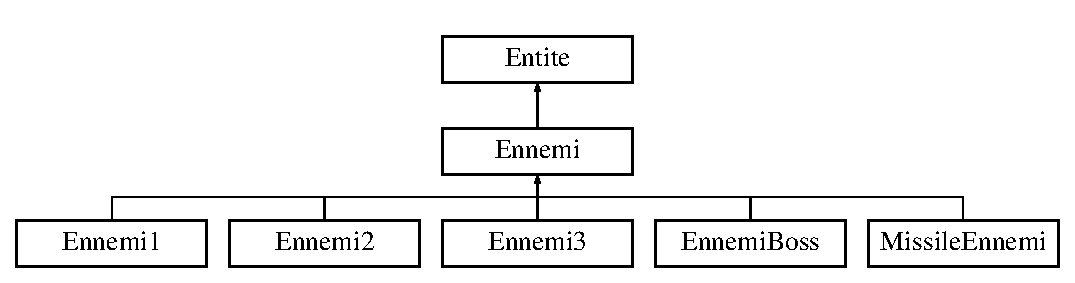
\includegraphics[height=3.000000cm]{class_ennemi}
\end{center}
\end{figure}
\subsection*{Public Member Functions}
\begin{DoxyCompactItemize}
\item 
\mbox{\Hypertarget{class_ennemi_a59b9815cc107dfed3eed6d33e7134d03}\label{class_ennemi_a59b9815cc107dfed3eed6d33e7134d03}} 
void {\bfseries deplacement} ()
\item 
\mbox{\Hypertarget{class_ennemi_ae7639e1f4294da03f07d07fc55c882bb}\label{class_ennemi_ae7639e1f4294da03f07d07fc55c882bb}} 
void \mbox{\hyperlink{class_ennemi_ae7639e1f4294da03f07d07fc55c882bb}{explosion\+Ennemi}} ()
\begin{DoxyCompactList}\small\item\em m�thode g�rant le d�placement des ennemis \end{DoxyCompactList}\item 
\mbox{\Hypertarget{class_ennemi_a522aca698f9b5042ddfdfe1b9ed35a0a}\label{class_ennemi_a522aca698f9b5042ddfdfe1b9ed35a0a}} 
void \mbox{\hyperlink{class_ennemi_a522aca698f9b5042ddfdfe1b9ed35a0a}{ennemi\+Hit}} ()
\begin{DoxyCompactList}\small\item\em Lorsqu\textquotesingle{}un ennemi n\textquotesingle{}a plus de PV, il explose. Cette m�thode permet de modifier le sprite de l\textquotesingle{}ennemi pour le transformer en explosion. \end{DoxyCompactList}\item 
\mbox{\Hypertarget{class_ennemi_a2dba94391ffa427ead3aa2688394342c}\label{class_ennemi_a2dba94391ffa427ead3aa2688394342c}} 
void \mbox{\hyperlink{class_ennemi_a2dba94391ffa427ead3aa2688394342c}{tirer}} ()
\begin{DoxyCompactList}\small\item\em Lorsqu\textquotesingle{}un ennemi est touch� mais a toujours PV$>$0, il clignote bri�vement en rouge. Cette m�thode modifie la couleur du sprite de l\textquotesingle{}ennemi avec la fonction S\+F\+ML .set\+Color() \end{DoxyCompactList}\end{DoxyCompactItemize}
\subsection*{Public Attributes}
\begin{DoxyCompactItemize}
\item 
\mbox{\Hypertarget{class_ennemi_ace453eadb96585c7dc37f7ee4dd04273}\label{class_ennemi_ace453eadb96585c7dc37f7ee4dd04273}} 
sf\+::\+Texture {\bfseries explosion}
\item 
\mbox{\Hypertarget{class_ennemi_acf8fb95ff9780d8b2e244de3999727d5}\label{class_ennemi_acf8fb95ff9780d8b2e244de3999727d5}} 
sf\+::\+Texture \mbox{\hyperlink{class_ennemi_acf8fb95ff9780d8b2e244de3999727d5}{texture}}
\begin{DoxyCompactList}\small\item\em Texture de l\textquotesingle{}explosion. \end{DoxyCompactList}\item 
\mbox{\Hypertarget{class_ennemi_a2953d1b46b7fad6b2ff40ff511bc3ee3}\label{class_ennemi_a2953d1b46b7fad6b2ff40ff511bc3ee3}} 
sf\+::\+Vector2f \mbox{\hyperlink{class_ennemi_a2953d1b46b7fad6b2ff40ff511bc3ee3}{pattern}}
\begin{DoxyCompactList}\small\item\em Texture normale de l\textquotesingle{}ennemi. \end{DoxyCompactList}\item 
\mbox{\Hypertarget{class_ennemi_a01bd46b3dcfe57606047fd625aa0723c}\label{class_ennemi_a01bd46b3dcfe57606047fd625aa0723c}} 
int \mbox{\hyperlink{class_ennemi_a01bd46b3dcfe57606047fd625aa0723c}{pv}}
\begin{DoxyCompactList}\small\item\em Vecteur de flottants contenant le mouvemlent de l\textquotesingle{}ennemi. \end{DoxyCompactList}\item 
\mbox{\Hypertarget{class_ennemi_a0d0cb59854e13d4e7b35385299d49f01}\label{class_ennemi_a0d0cb59854e13d4e7b35385299d49f01}} 
int \mbox{\hyperlink{class_ennemi_a0d0cb59854e13d4e7b35385299d49f01}{points}}
\begin{DoxyCompactList}\small\item\em Nombre de points de vie de l\textquotesingle{}ennemi. \end{DoxyCompactList}\item 
\mbox{\Hypertarget{class_ennemi_acbf0a832ef05cb5710ebb3770b9b4712}\label{class_ennemi_acbf0a832ef05cb5710ebb3770b9b4712}} 
bool \mbox{\hyperlink{class_ennemi_acbf0a832ef05cb5710ebb3770b9b4712}{boom}} = false
\begin{DoxyCompactList}\small\item\em Points rapport�s au joueur lorsque l\textquotesingle{}ennemi est d�truit. \end{DoxyCompactList}\item 
\mbox{\Hypertarget{class_ennemi_aa4ef3ea57356bb41feb3b45438e4f1ce}\label{class_ennemi_aa4ef3ea57356bb41feb3b45438e4f1ce}} 
bool {\bfseries incr\+Score} = true
\item 
\mbox{\Hypertarget{class_ennemi_a907151bfeaabc72f7cb6cfb6d9e14bb3}\label{class_ennemi_a907151bfeaabc72f7cb6cfb6d9e14bb3}} 
bool {\bfseries d�gats\+Joueur} = true
\item 
\mbox{\Hypertarget{class_ennemi_a55e5947385d10b7ef1f94417fffb63e9}\label{class_ennemi_a55e5947385d10b7ef1f94417fffb63e9}} 
bool \mbox{\hyperlink{class_ennemi_a55e5947385d10b7ef1f94417fffb63e9}{move}} = true
\begin{DoxyCompactList}\small\item\em Lorsque ce bool�en est T\+R\+UE, l\textquotesingle{}ennemi inflige des d�gats au joueur lorsqu\textquotesingle{}il y a collision. \end{DoxyCompactList}\item 
\mbox{\Hypertarget{class_ennemi_ae3d34c3d9b246593f781347adacc1f3a}\label{class_ennemi_ae3d34c3d9b246593f781347adacc1f3a}} 
bool \mbox{\hyperlink{class_ennemi_ae3d34c3d9b246593f781347adacc1f3a}{hit}} = false
\begin{DoxyCompactList}\small\item\em ce bool�en est utilis� afin de bloquer le mouvement de l\textquotesingle{}ennemi lorsque ses PV=0 afin que le sprite de son explosion ne se d�place pas \end{DoxyCompactList}\item 
\mbox{\Hypertarget{class_ennemi_ad9c73f7fec8685d9d558d2c518b8e099}\label{class_ennemi_ad9c73f7fec8685d9d558d2c518b8e099}} 
bool {\bfseries shoot} = false
\item 
\mbox{\Hypertarget{class_ennemi_ac83f632da93cda2d5fc90752af0a0abc}\label{class_ennemi_ac83f632da93cda2d5fc90752af0a0abc}} 
bool \mbox{\hyperlink{class_ennemi_ac83f632da93cda2d5fc90752af0a0abc}{tir\+Ok}} = false
\begin{DoxyCompactList}\small\item\em lorsque shoot = true, l\textquotesingle{}ennemi tire \end{DoxyCompactList}\item 
\mbox{\Hypertarget{class_ennemi_ac26fe5ce582430a726ab29997258643e}\label{class_ennemi_ac26fe5ce582430a726ab29997258643e}} 
bool \mbox{\hyperlink{class_ennemi_ac26fe5ce582430a726ab29997258643e}{S\+FX}} = true
\begin{DoxyCompactList}\small\item\em ce bool�en est utilis� afin d\textquotesingle{}activer le tir depuis une autre classe \end{DoxyCompactList}\item 
\mbox{\Hypertarget{class_ennemi_a8b6d22ecf4d65cff6cd9735d7497ace1}\label{class_ennemi_a8b6d22ecf4d65cff6cd9735d7497ace1}} 
float {\bfseries inc} = 0
\item 
\mbox{\Hypertarget{class_ennemi_a6a4f426faa99e8f5e74b6a4c45eea9e8}\label{class_ennemi_a6a4f426faa99e8f5e74b6a4c45eea9e8}} 
sf\+::\+Clock \mbox{\hyperlink{class_ennemi_a6a4f426faa99e8f5e74b6a4c45eea9e8}{clock\+Hit}}
\begin{DoxyCompactList}\small\item\em variable d\textquotesingle{}incr�mentation utilis�e dans l\textquotesingle{}animation de l\textquotesingle{}explosion, permet de passer d\textquotesingle{}une frame d\textquotesingle{}animation � une autre gr�ce � une incr�mantation de 14px \end{DoxyCompactList}\item 
\mbox{\Hypertarget{class_ennemi_a6bbe605d71452836b42e94ef8cf9fe45}\label{class_ennemi_a6bbe605d71452836b42e94ef8cf9fe45}} 
sf\+::\+Clock \mbox{\hyperlink{class_ennemi_a6bbe605d71452836b42e94ef8cf9fe45}{clock\+Explosion}}
\begin{DoxyCompactList}\small\item\em Permet de g�rer la dur�e de la fonction ennemi\+Hit. \end{DoxyCompactList}\item 
\mbox{\Hypertarget{class_ennemi_a02b4351e7babcecf911f1554b593be79}\label{class_ennemi_a02b4351e7babcecf911f1554b593be79}} 
sf\+::\+Clock \mbox{\hyperlink{class_ennemi_a02b4351e7babcecf911f1554b593be79}{missile\+Clock}}
\begin{DoxyCompactList}\small\item\em Clock g�rant l\textquotesingle{}animation de l\textquotesingle{}explosion. \end{DoxyCompactList}\item 
\mbox{\Hypertarget{class_ennemi_a3fbc750432c43e977808d3b4a96f7f75}\label{class_ennemi_a3fbc750432c43e977808d3b4a96f7f75}} 
int {\bfseries vitesse\+Tir}
\end{DoxyCompactItemize}


\subsection{Detailed Description}
Classe de cr�ation des vaisseaux ennemis. 

The documentation for this class was generated from the following files\+:\begin{DoxyCompactItemize}
\item 
prog/Ennemi.\+h\item 
prog/Ennemi.\+cpp\end{DoxyCompactItemize}

\hypertarget{class_ennemi1}{}\section{Ennemi1 Class Reference}
\label{class_ennemi1}\index{Ennemi1@{Ennemi1}}
Inheritance diagram for Ennemi1\+:\begin{figure}[H]
\begin{center}
\leavevmode
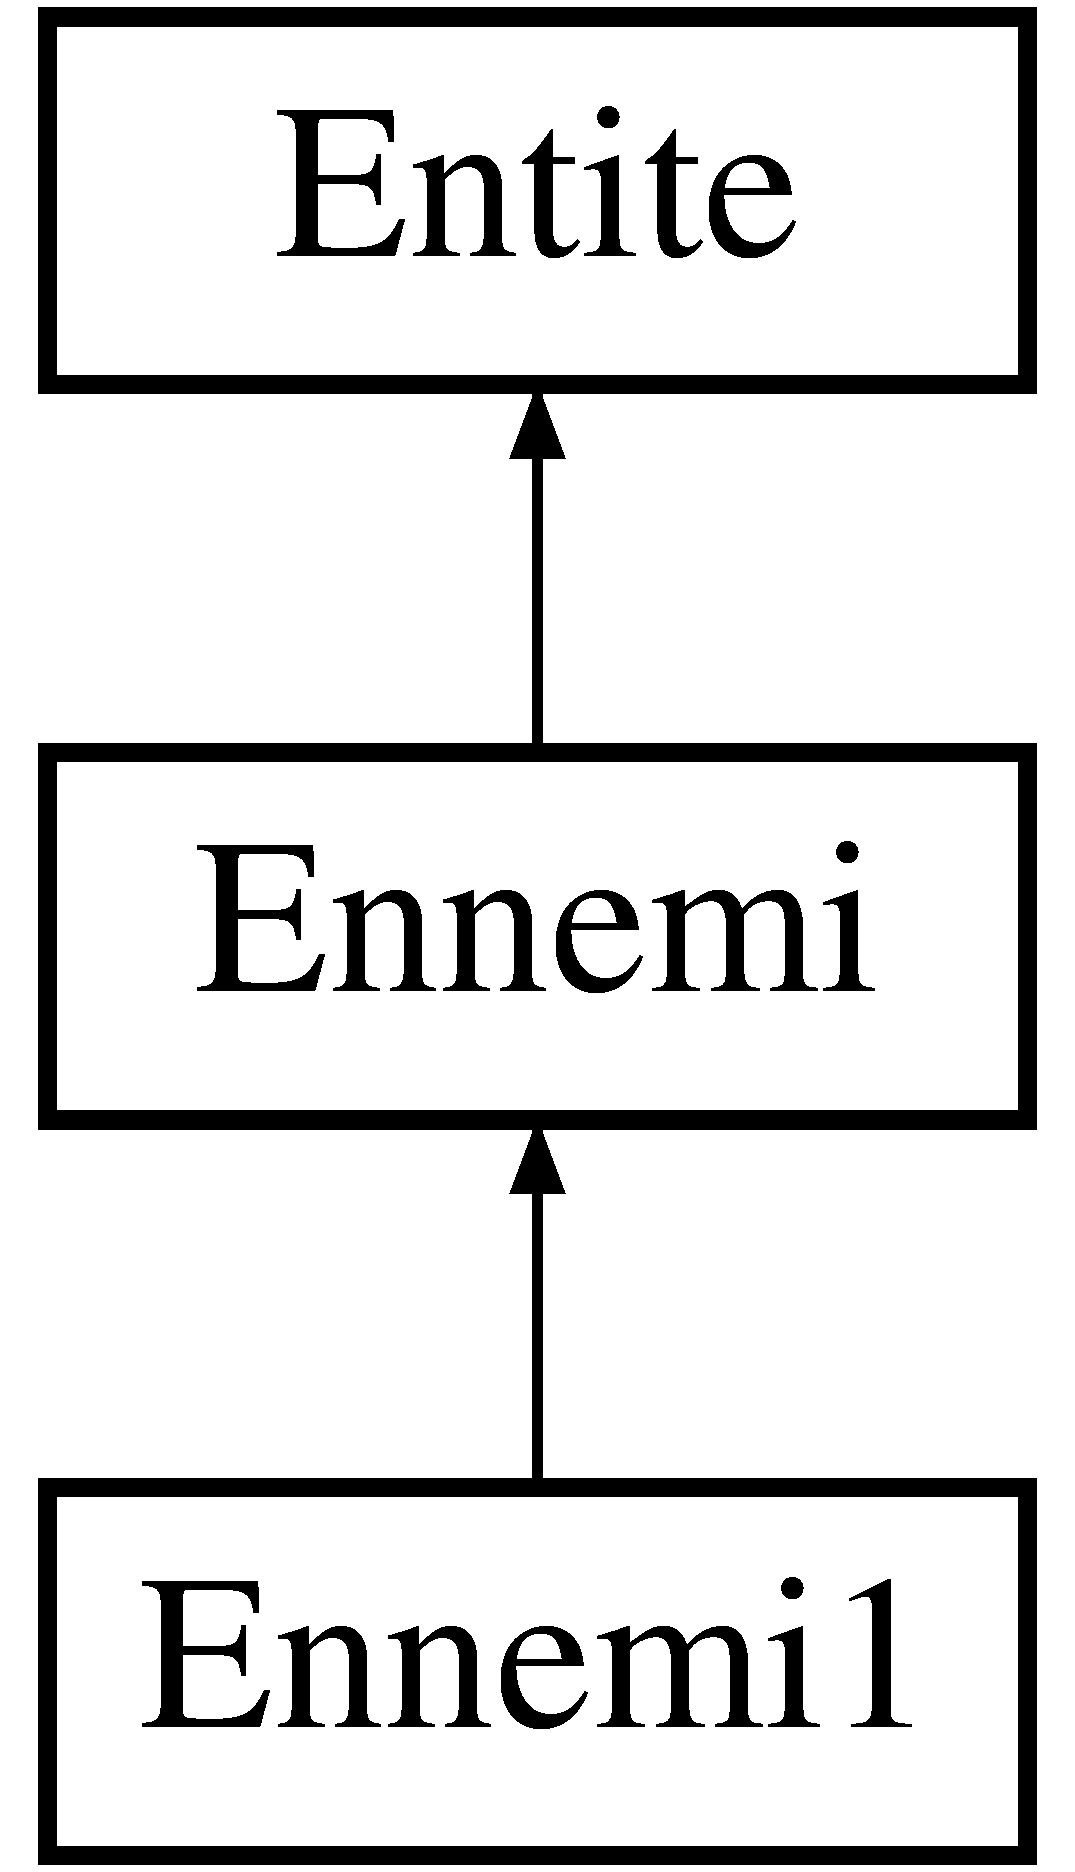
\includegraphics[height=3.000000cm]{class_ennemi1}
\end{center}
\end{figure}
\subsection*{Additional Inherited Members}


The documentation for this class was generated from the following files\+:\begin{DoxyCompactItemize}
\item 
prog/Ennemi1.\+h\item 
prog/Ennemi1.\+cpp\end{DoxyCompactItemize}

\hypertarget{class_ennemi2}{}\section{Ennemi2 Class Reference}
\label{class_ennemi2}\index{Ennemi2@{Ennemi2}}
Inheritance diagram for Ennemi2\+:\begin{figure}[H]
\begin{center}
\leavevmode
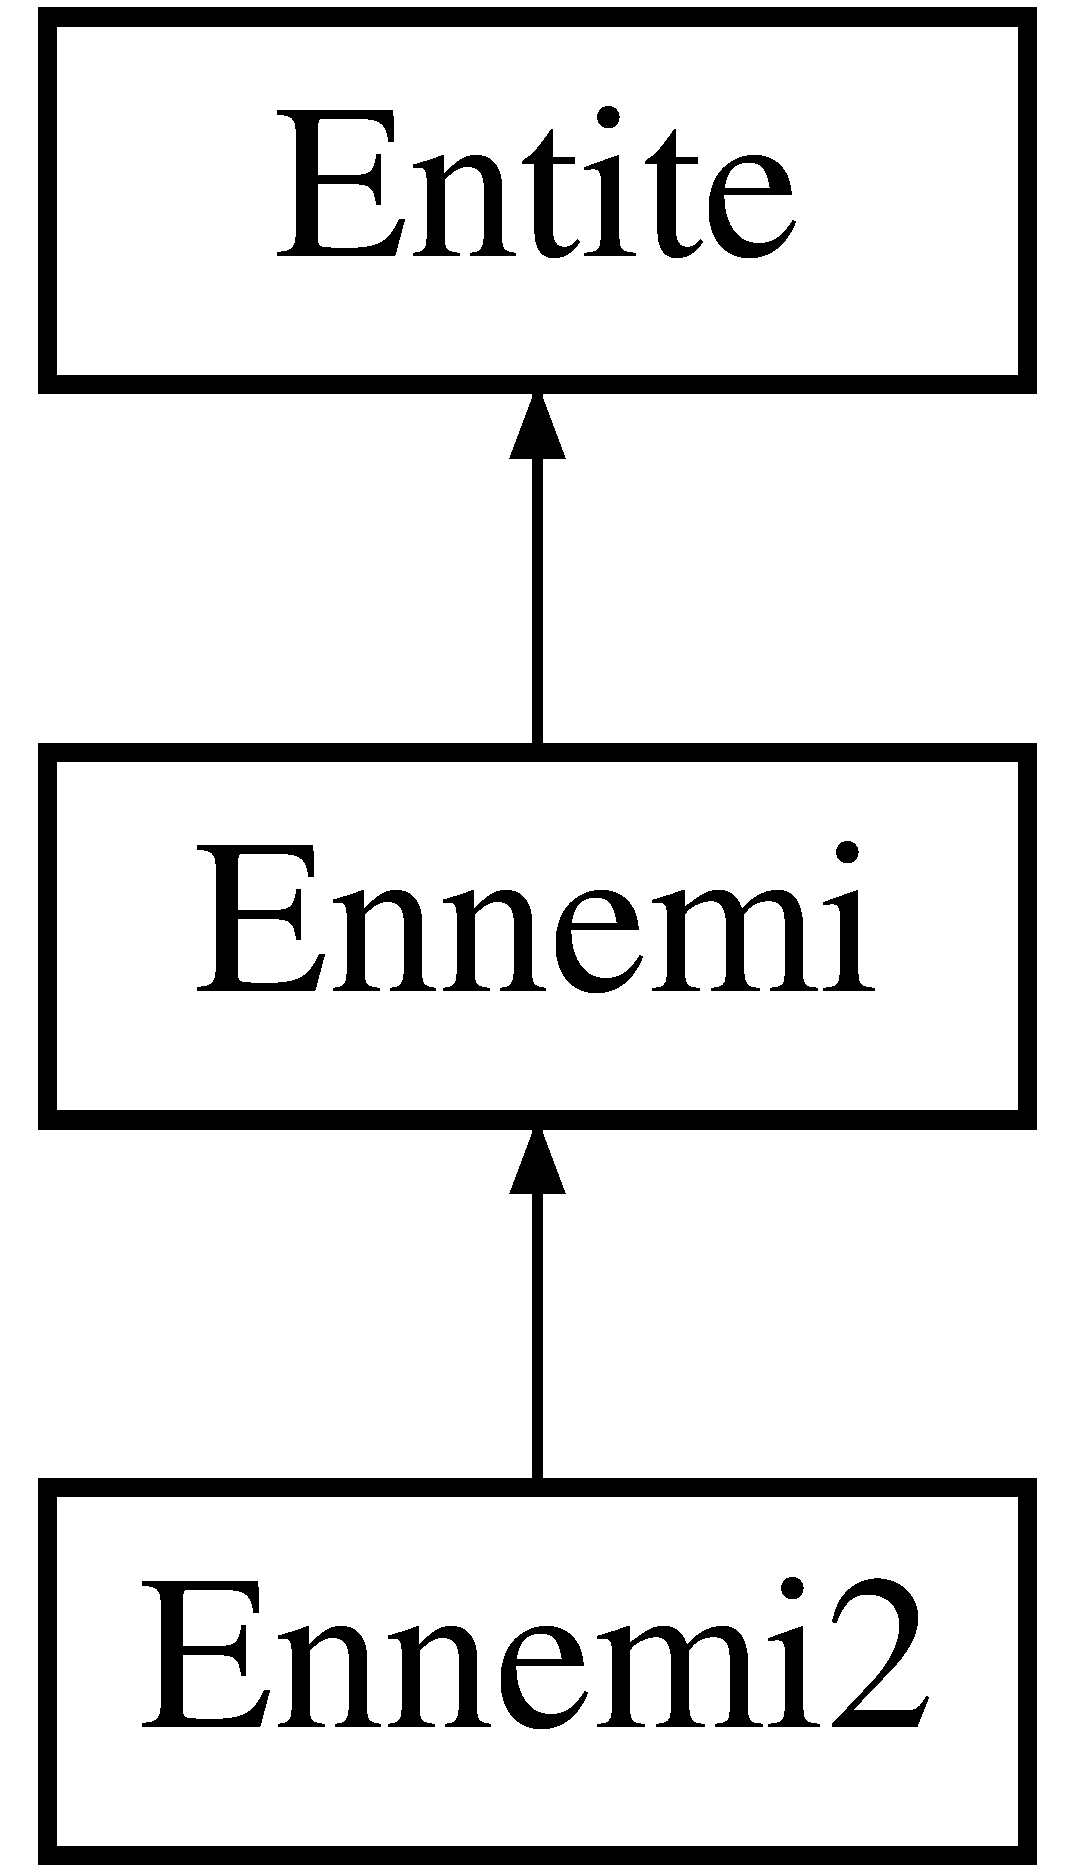
\includegraphics[height=3.000000cm]{class_ennemi2}
\end{center}
\end{figure}
\subsection*{Public Attributes}
\begin{DoxyCompactItemize}
\item 
\mbox{\Hypertarget{class_ennemi2_ac1586963ba5375fbba7f9483d0393b35}\label{class_ennemi2_ac1586963ba5375fbba7f9483d0393b35}} 
sf\+::\+Texture {\bfseries texture2}
\end{DoxyCompactItemize}
\subsection*{Additional Inherited Members}


The documentation for this class was generated from the following files\+:\begin{DoxyCompactItemize}
\item 
prog/Ennemi2.\+h\item 
prog/Ennemi2.\+cpp\end{DoxyCompactItemize}

\hypertarget{class_ennemi3}{}\section{Ennemi3 Class Reference}
\label{class_ennemi3}\index{Ennemi3@{Ennemi3}}
Inheritance diagram for Ennemi3\+:\begin{figure}[H]
\begin{center}
\leavevmode
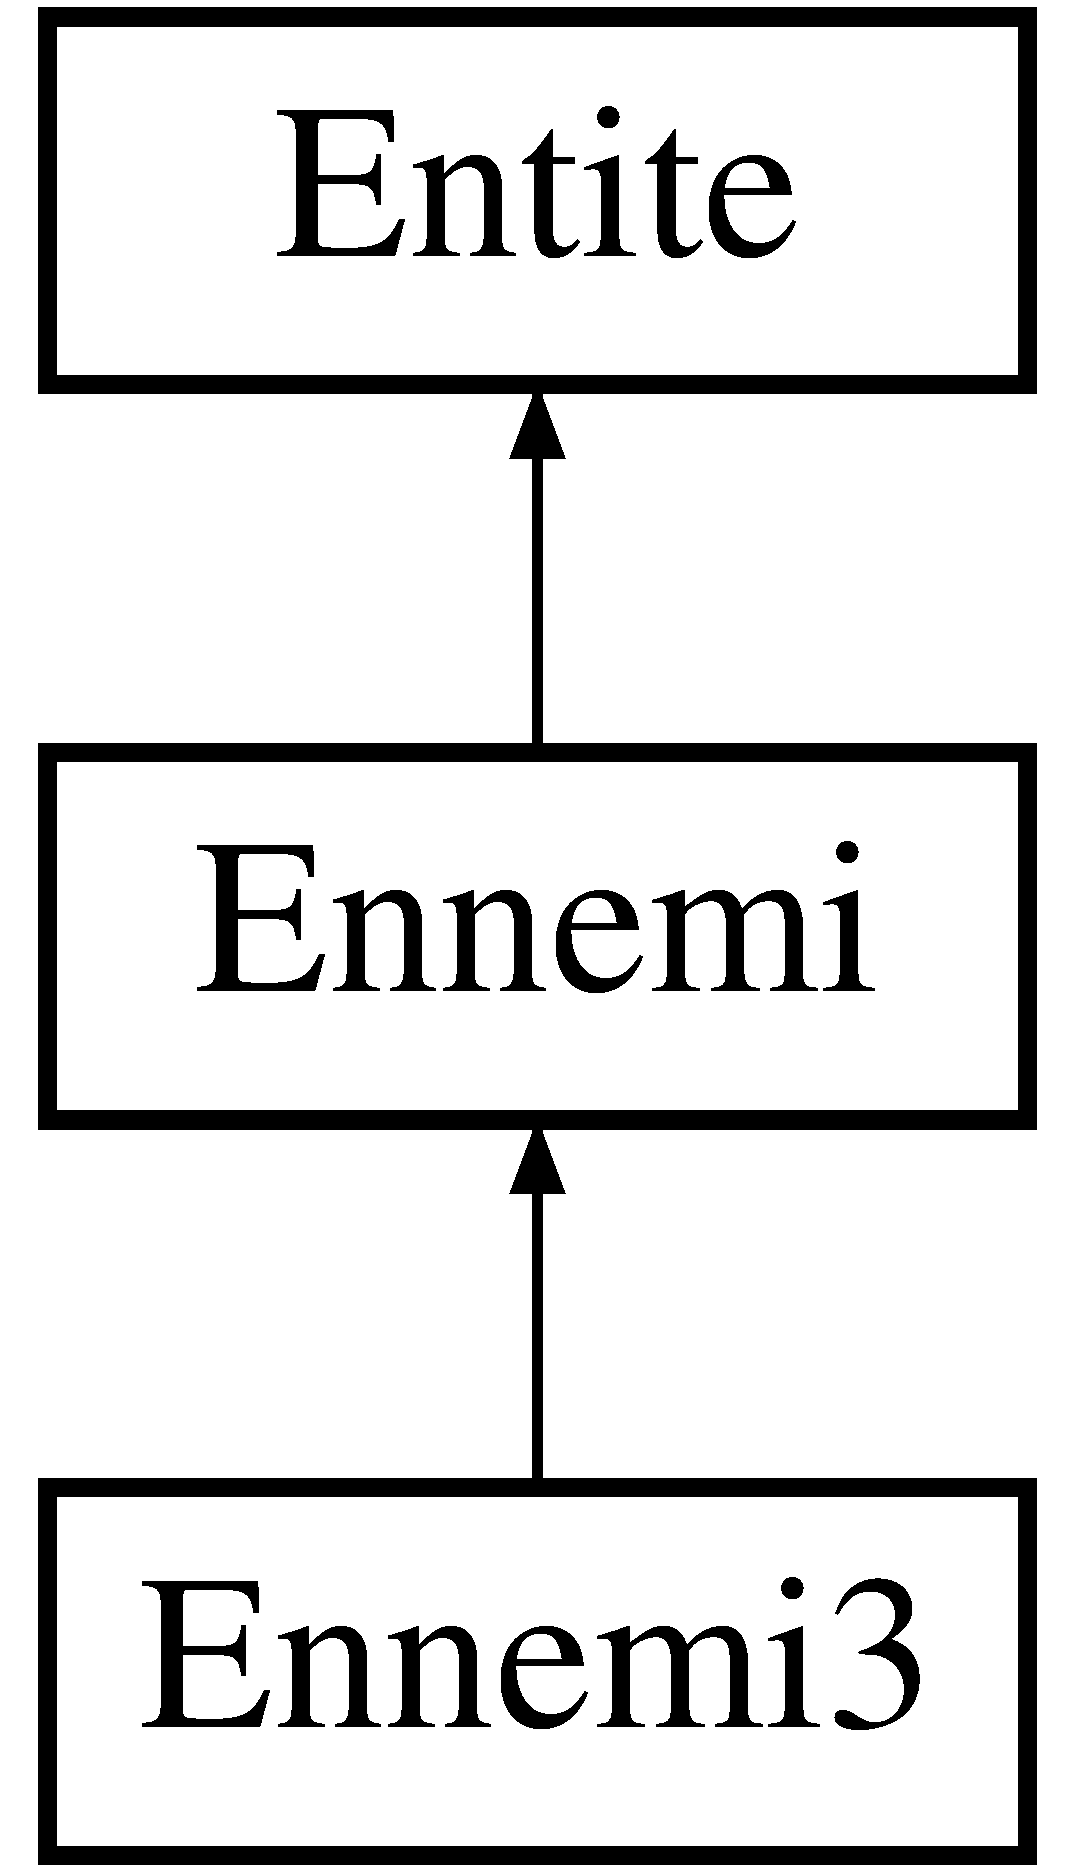
\includegraphics[height=3.000000cm]{class_ennemi3}
\end{center}
\end{figure}
\subsection*{Additional Inherited Members}


The documentation for this class was generated from the following files\+:\begin{DoxyCompactItemize}
\item 
prog/Ennemi3.\+h\item 
prog/Ennemi3.\+cpp\end{DoxyCompactItemize}

\hypertarget{class_ennemi_boss}{}\section{Ennemi\+Boss Class Reference}
\label{class_ennemi_boss}\index{Ennemi\+Boss@{Ennemi\+Boss}}
Inheritance diagram for Ennemi\+Boss\+:\begin{figure}[H]
\begin{center}
\leavevmode
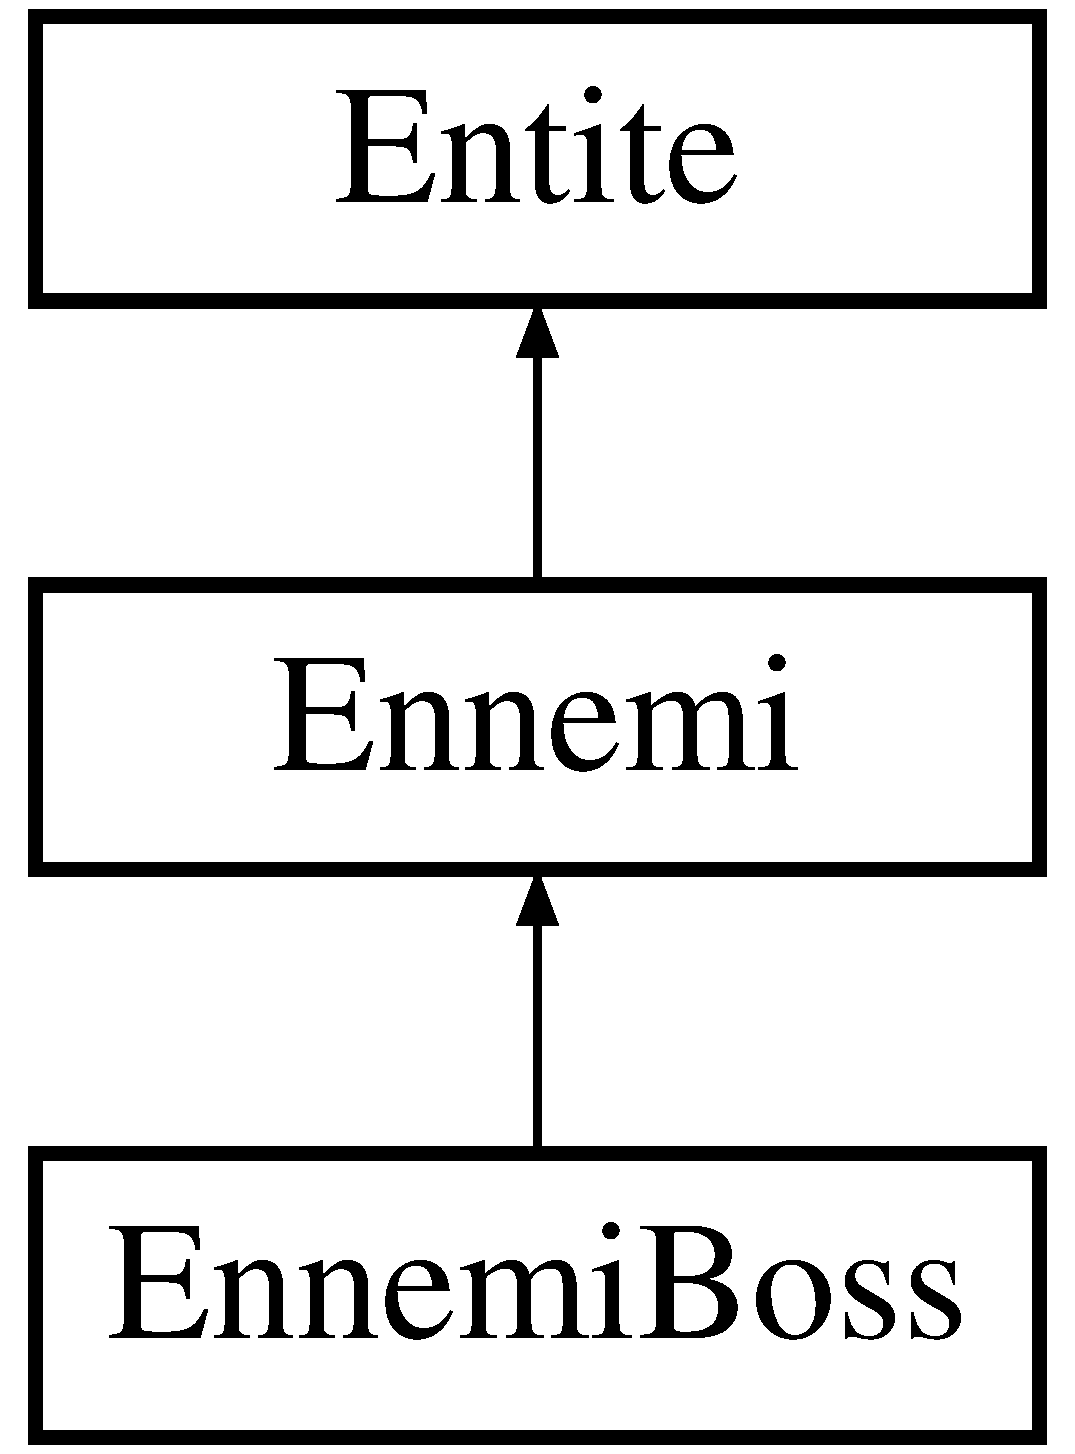
\includegraphics[height=3.000000cm]{class_ennemi_boss}
\end{center}
\end{figure}
\subsection*{Public Attributes}
\begin{DoxyCompactItemize}
\item 
\mbox{\Hypertarget{class_ennemi_boss_a98ffff45074e0f9a79ecf8d60e7b5af1}\label{class_ennemi_boss_a98ffff45074e0f9a79ecf8d60e7b5af1}} 
sf\+::\+Texture {\bfseries texture2}
\end{DoxyCompactItemize}
\subsection*{Additional Inherited Members}


The documentation for this class was generated from the following files\+:\begin{DoxyCompactItemize}
\item 
prog/Ennemi\+Boss.\+h\item 
prog/Ennemi\+Boss.\+cpp\end{DoxyCompactItemize}

\hypertarget{classenregistrement_b_d_d}{}\section{enregistrement\+B\+DD Class Reference}
\label{classenregistrement_b_d_d}\index{enregistrement\+B\+DD@{enregistrement\+B\+DD}}


Cette classe permet de cr�er un objet qui facilite la r�cup�ration des donn�es dans la \mbox{\hyperlink{class_b_d_d}{B\+DD}}.  




{\ttfamily \#include $<$enregistrement\+B\+D\+D.\+h$>$}

\subsection*{Public Attributes}
\begin{DoxyCompactItemize}
\item 
\mbox{\Hypertarget{classenregistrement_b_d_d_ac9e6bea1f6922410d7102f5c4447bfd7}\label{classenregistrement_b_d_d_ac9e6bea1f6922410d7102f5c4447bfd7}} 
std\+::string {\bfseries nom}
\item 
\mbox{\Hypertarget{classenregistrement_b_d_d_a61b56e584053b9c6801d524ab5e32738}\label{classenregistrement_b_d_d_a61b56e584053b9c6801d524ab5e32738}} 
int \mbox{\hyperlink{classenregistrement_b_d_d_a61b56e584053b9c6801d524ab5e32738}{score}}
\begin{DoxyCompactList}\small\item\em Nom � r�cup�rer. \end{DoxyCompactList}\end{DoxyCompactItemize}


\subsection{Detailed Description}
Cette classe permet de cr�er un objet qui facilite la r�cup�ration des donn�es dans la \mbox{\hyperlink{class_b_d_d}{B\+DD}}. 

The documentation for this class was generated from the following files\+:\begin{DoxyCompactItemize}
\item 
prog/enregistrement\+B\+D\+D.\+h\item 
prog/enregistrement\+B\+D\+D.\+cpp\end{DoxyCompactItemize}

\hypertarget{class_entite}{}\section{Entite Class Reference}
\label{class_entite}\index{Entite@{Entite}}


Cette classe est la base de la plupart des objets cr��s dans le jeu. Elle poss�de un sprite et une forme.  




{\ttfamily \#include $<$Entite.\+h$>$}

Inheritance diagram for Entite\+:\begin{figure}[H]
\begin{center}
\leavevmode
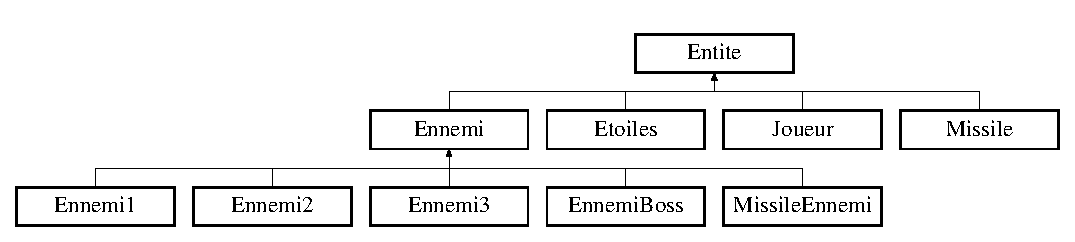
\includegraphics[height=2.800000cm]{class_entite}
\end{center}
\end{figure}
\subsection*{Public Attributes}
\begin{DoxyCompactItemize}
\item 
\mbox{\Hypertarget{class_entite_adb1c7d77d4d8b6d5b46d1cd3ac033b57}\label{class_entite_adb1c7d77d4d8b6d5b46d1cd3ac033b57}} 
sf\+::\+Sprite {\bfseries sprite}
\item 
\mbox{\Hypertarget{class_entite_acd57e84d2aa82b3aae8a262ebdf902b4}\label{class_entite_acd57e84d2aa82b3aae8a262ebdf902b4}} 
sf\+::\+Rectangle\+Shape \mbox{\hyperlink{class_entite_acd57e84d2aa82b3aae8a262ebdf902b4}{forme}}
\begin{DoxyCompactList}\small\item\em Sprite de l\textquotesingle{}entit� (pour ennemis/joueur) \end{DoxyCompactList}\item 
\mbox{\Hypertarget{class_entite_a72dcc7c6ea83fcb9a65e42230798c6c0}\label{class_entite_a72dcc7c6ea83fcb9a65e42230798c6c0}} 
sf\+::\+Circle\+Shape \mbox{\hyperlink{class_entite_a72dcc7c6ea83fcb9a65e42230798c6c0}{cercle}}
\begin{DoxyCompactList}\small\item\em forme rectangulaire (pour les projectiles, bordures) \end{DoxyCompactList}\end{DoxyCompactItemize}


\subsection{Detailed Description}
Cette classe est la base de la plupart des objets cr��s dans le jeu. Elle poss�de un sprite et une forme. 

The documentation for this class was generated from the following files\+:\begin{DoxyCompactItemize}
\item 
prog/Entite.\+h\item 
prog/Entite.\+cpp\end{DoxyCompactItemize}

\hypertarget{class_etoiles}{}\section{Etoiles Class Reference}
\label{class_etoiles}\index{Etoiles@{Etoiles}}


Permet la cr�ation des �toiles pour le background.  




{\ttfamily \#include $<$Etoiles.\+h$>$}

Inheritance diagram for Etoiles\+:\begin{figure}[H]
\begin{center}
\leavevmode
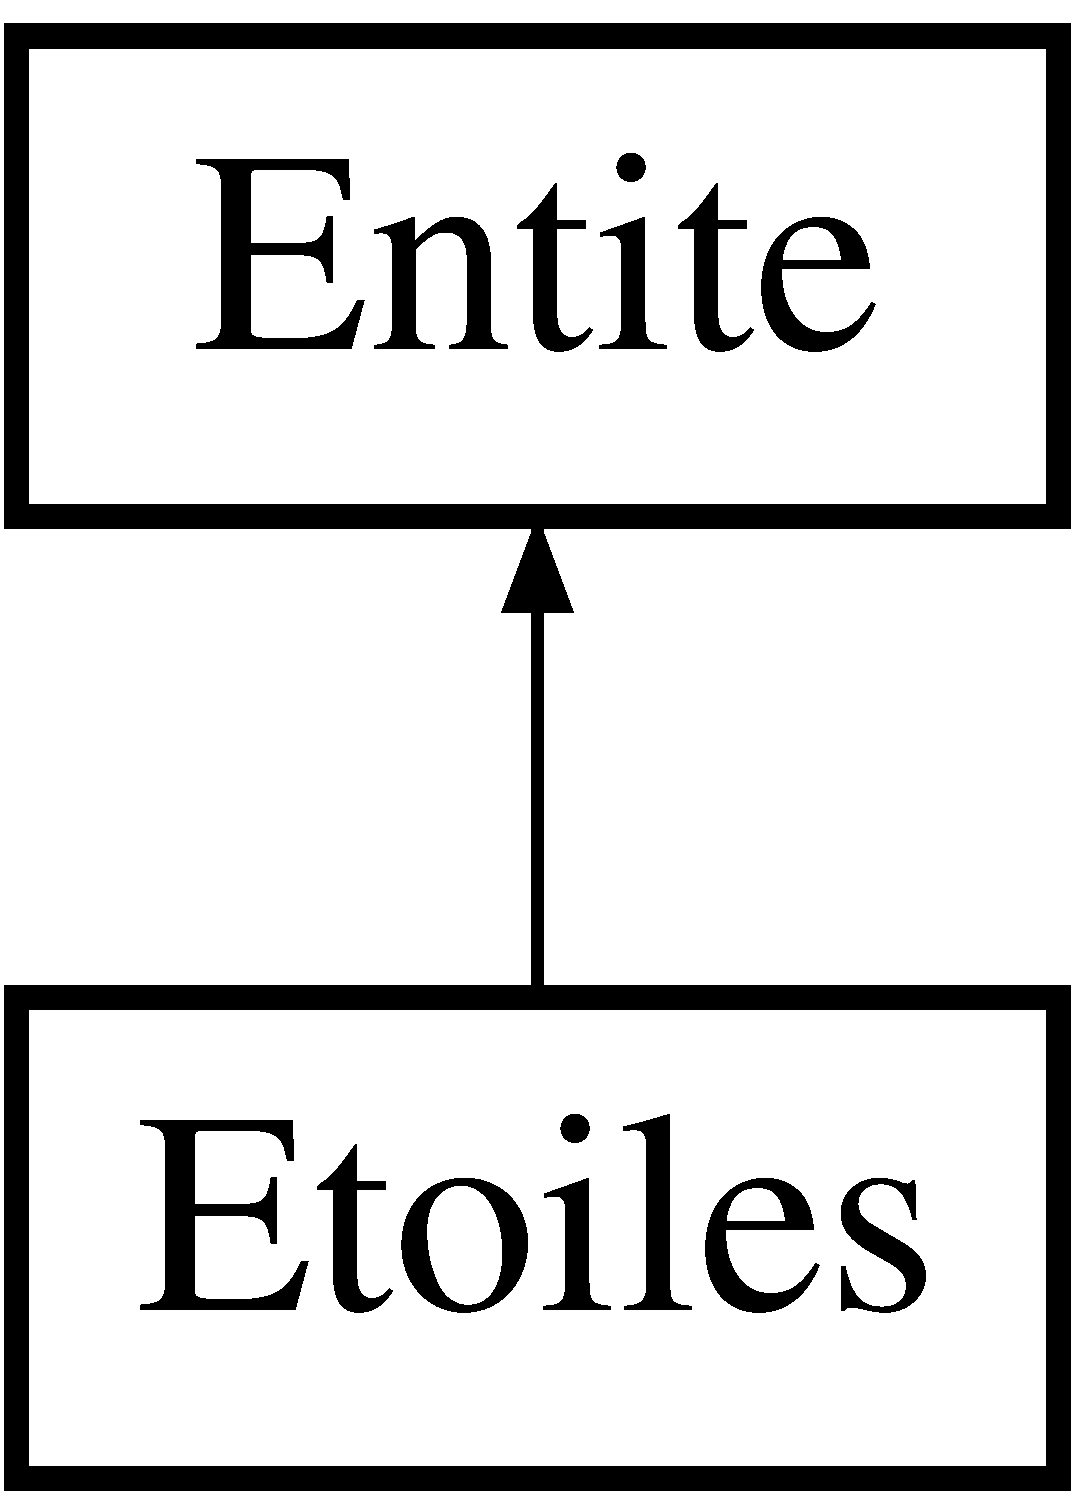
\includegraphics[height=2.000000cm]{class_etoiles}
\end{center}
\end{figure}
\subsection*{Public Member Functions}
\begin{DoxyCompactItemize}
\item 
\mbox{\Hypertarget{class_etoiles_afc86cbf9c7f1e6c0f13439159aaf7878}\label{class_etoiles_afc86cbf9c7f1e6c0f13439159aaf7878}} 
{\bfseries Etoiles} (sf\+::\+Color couleur, float vitesse)
\end{DoxyCompactItemize}
\subsection*{Public Attributes}
\begin{DoxyCompactItemize}
\item 
\mbox{\Hypertarget{class_etoiles_a51a5dd1b22293dcb74a00bc4a51976ae}\label{class_etoiles_a51a5dd1b22293dcb74a00bc4a51976ae}} 
float {\bfseries vitesse}
\end{DoxyCompactItemize}


\subsection{Detailed Description}
Permet la cr�ation des �toiles pour le background. 

The documentation for this class was generated from the following files\+:\begin{DoxyCompactItemize}
\item 
prog/Etoiles.\+h\item 
prog/Etoiles.\+cpp\end{DoxyCompactItemize}

\hypertarget{class_explosion}{}\section{Explosion Class Reference}
\label{class_explosion}\index{Explosion@{Explosion}}


Gestion des explosions du joueur et de la m�ga bombe.  




{\ttfamily \#include $<$Explosion.\+h$>$}

\subsection*{Public Member Functions}
\begin{DoxyCompactItemize}
\item 
\mbox{\Hypertarget{class_explosion_acb09fbd696591a363671dfee27527ecd}\label{class_explosion_acb09fbd696591a363671dfee27527ecd}} 
{\bfseries Explosion} (int scale)
\item 
\mbox{\Hypertarget{class_explosion_ac9c0baa7268ff5b8f4f358074a1326c0}\label{class_explosion_ac9c0baa7268ff5b8f4f358074a1326c0}} 
\mbox{\hyperlink{class_explosion_ac9c0baa7268ff5b8f4f358074a1326c0}{$\sim$\+Explosion}} ()
\begin{DoxyCompactList}\small\item\em constructeur avec en param�tre l\textquotesingle{}�chelle de l\textquotesingle{}explosion (taille) \end{DoxyCompactList}\item 
\mbox{\Hypertarget{class_explosion_afd94e6cebd1eb1893d073260ed971490}\label{class_explosion_afd94e6cebd1eb1893d073260ed971490}} 
void {\bfseries animation} ()
\end{DoxyCompactItemize}
\subsection*{Public Attributes}
\begin{DoxyCompactItemize}
\item 
\mbox{\Hypertarget{class_explosion_a57ac8dd2eb0dd054fde43fa806071dd3}\label{class_explosion_a57ac8dd2eb0dd054fde43fa806071dd3}} 
int \mbox{\hyperlink{class_explosion_a57ac8dd2eb0dd054fde43fa806071dd3}{inc}} = 0
\begin{DoxyCompactList}\small\item\em fonction g�rant l\textquotesingle{}animation de l\textquotesingle{}explosion \end{DoxyCompactList}\item 
\mbox{\Hypertarget{class_explosion_a60f51e1055082b5db9730dfe84a26737}\label{class_explosion_a60f51e1055082b5db9730dfe84a26737}} 
sf\+::\+Clock \mbox{\hyperlink{class_explosion_a60f51e1055082b5db9730dfe84a26737}{clock}}
\begin{DoxyCompactList}\small\item\em variable d\textquotesingle{}incr�mentation, utilis�e pour l\textquotesingle{}animation \end{DoxyCompactList}\item 
\mbox{\Hypertarget{class_explosion_adbf69b5bfa9582a1f935fc5a6f39995b}\label{class_explosion_adbf69b5bfa9582a1f935fc5a6f39995b}} 
bool \mbox{\hyperlink{class_explosion_adbf69b5bfa9582a1f935fc5a6f39995b}{trigger}}
\begin{DoxyCompactList}\small\item\em Clock utilis�e pour l\textquotesingle{}animation de l\textquotesingle{}explosion. \end{DoxyCompactList}\item 
\mbox{\Hypertarget{class_explosion_a4d8ca9db59b67ca2bdfc7eeab4acc48b}\label{class_explosion_a4d8ca9db59b67ca2bdfc7eeab4acc48b}} 
sf\+::\+Texture {\bfseries texture\+Explosion}
\item 
\mbox{\Hypertarget{class_explosion_a364287e696d02c023b4a2437d3f479aa}\label{class_explosion_a364287e696d02c023b4a2437d3f479aa}} 
sf\+::\+Sprite \mbox{\hyperlink{class_explosion_a364287e696d02c023b4a2437d3f479aa}{explosion}}
\begin{DoxyCompactList}\small\item\em texture de l\textquotesingle{}explosion \end{DoxyCompactList}\end{DoxyCompactItemize}


\subsection{Detailed Description}
Gestion des explosions du joueur et de la m�ga bombe. 

The documentation for this class was generated from the following files\+:\begin{DoxyCompactItemize}
\item 
prog/Explosion.\+h\item 
prog/Explosion.\+cpp\end{DoxyCompactItemize}

\hypertarget{class_game}{}\section{Game Class Reference}
\label{class_game}\index{Game@{Game}}


Cette classe g�re la logique des �vennements du jeu et l\textquotesingle{}affichage.  




{\ttfamily \#include $<$Game.\+h$>$}

\subsection*{Public Member Functions}
\begin{DoxyCompactItemize}
\item 
void \mbox{\hyperlink{class_game_a3780dd03ab98d082bae2a86733c364fe}{logique\+Du\+Jeu}} ()
\end{DoxyCompactItemize}
\subsection*{Public Attributes}
\begin{DoxyCompactItemize}
\item 
\mbox{\Hypertarget{class_game_ac5aa2df49b05977a8993a05f547171d4}\label{class_game_ac5aa2df49b05977a8993a05f547171d4}} 
\mbox{\hyperlink{class_niveaux}{Niveaux}} \mbox{\hyperlink{class_game_ac5aa2df49b05977a8993a05f547171d4}{niveaux}}
\begin{DoxyCompactList}\small\item\em Fonction principale g�rant toute la logique et l\textquotesingle{}affichage. \end{DoxyCompactList}\item 
float \mbox{\hyperlink{class_game_a75266462970ce3f9897f99d5d52adf6e}{rouge}} = 20
\begin{DoxyCompactList}\small\item\em Appel � la classe \mbox{\hyperlink{class_niveaux}{Niveaux}} quiposs�de toutes les m�thodes pour cr�er plus facilement des niveaux. \end{DoxyCompactList}\item 
\mbox{\Hypertarget{class_game_a71a87b7fb8885bc0f34c477a370bb502}\label{class_game_a71a87b7fb8885bc0f34c477a370bb502}} 
float \mbox{\hyperlink{class_game_a71a87b7fb8885bc0f34c477a370bb502}{vert}} = 20
\begin{DoxyCompactList}\small\item\em variable utilis�e pour modifier la couleur rouge de l\textquotesingle{}arri�re plan \end{DoxyCompactList}\item 
\mbox{\Hypertarget{class_game_a0e8d717d871802cf43d88bfcf063dc8d}\label{class_game_a0e8d717d871802cf43d88bfcf063dc8d}} 
float \mbox{\hyperlink{class_game_a0e8d717d871802cf43d88bfcf063dc8d}{bleu}} = 20
\begin{DoxyCompactList}\small\item\em variable utilis�e pour modifier la couleur verte de l\textquotesingle{}arri�re plan \end{DoxyCompactList}\item 
\mbox{\Hypertarget{class_game_a7be5c4d5161e4f8c060d84890543832d}\label{class_game_a7be5c4d5161e4f8c060d84890543832d}} 
bool \mbox{\hyperlink{class_game_a7be5c4d5161e4f8c060d84890543832d}{go\+On}} = false
\begin{DoxyCompactList}\small\item\em variable utilis�e pour modifier la couleur bleue de l\textquotesingle{}arri�re plan \end{DoxyCompactList}\item 
\mbox{\Hypertarget{class_game_a2cd2b5e465e5820e90ef108258ac982c}\label{class_game_a2cd2b5e465e5820e90ef108258ac982c}} 
bool \mbox{\hyperlink{class_game_a2cd2b5e465e5820e90ef108258ac982c}{pause}} = false
\begin{DoxyCompactList}\small\item\em go\+On = false emp�che le joueur de passer � un autre �tat du jeu \end{DoxyCompactList}\item 
\mbox{\Hypertarget{class_game_ad5ca493c9de125e428395fb7ef066170}\label{class_game_ad5ca493c9de125e428395fb7ef066170}} 
int {\bfseries niveau\+En\+Cours} = 0
\item 
\mbox{\Hypertarget{class_game_ab3691a278f20a82fd92b3dc490e892ea}\label{class_game_ab3691a278f20a82fd92b3dc490e892ea}} 
sf\+::\+Clock \mbox{\hyperlink{class_game_ab3691a278f20a82fd92b3dc490e892ea}{temps}}
\begin{DoxyCompactList}\small\item\em Variable permettant de d�lectionner le niveaux. \end{DoxyCompactList}\item 
\mbox{\Hypertarget{class_game_a3bcd561d881779233a4975a4bcad8b8b}\label{class_game_a3bcd561d881779233a4975a4bcad8b8b}} 
sf\+::\+Clock \mbox{\hyperlink{class_game_a3bcd561d881779233a4975a4bcad8b8b}{temps\+Titre}}
\begin{DoxyCompactList}\small\item\em horloge principale du jeu \end{DoxyCompactList}\item 
\mbox{\Hypertarget{class_game_a7c0c44c3c1e97931bb31b10daf76ef92}\label{class_game_a7c0c44c3c1e97931bb31b10daf76ef92}} 
sf\+::\+Clock \mbox{\hyperlink{class_game_a7c0c44c3c1e97931bb31b10daf76ef92}{frame}}
\begin{DoxyCompactList}\small\item\em horloge utilis�e pendant l\textquotesingle{}�cran titre \end{DoxyCompactList}\item 
sf\+::\+Vector2f \mbox{\hyperlink{class_game_a36bd909275412072a7596cabcb686340}{position\+Precedente}}
\begin{DoxyCompactList}\small\item\em pour le calcul du frame rate \end{DoxyCompactList}\item 
sf\+::\+Clock \mbox{\hyperlink{class_game_a573e866c506a1b59880a202e00585dad}{cadence\+Canon}}
\begin{DoxyCompactList}\small\item\em armes du joueur \end{DoxyCompactList}\item 
\mbox{\Hypertarget{class_game_a5ca0d0c721b9afc9628cb1b0851a433b}\label{class_game_a5ca0d0c721b9afc9628cb1b0851a433b}} 
sf\+::\+Clock \mbox{\hyperlink{class_game_a5ca0d0c721b9afc9628cb1b0851a433b}{temps\+Activation\+Canon}}
\begin{DoxyCompactList}\small\item\em clock pour g�rer la vitesse du canon \end{DoxyCompactList}\item 
\mbox{\Hypertarget{class_game_ac03125de12d79747c6203a3f8477fb08}\label{class_game_ac03125de12d79747c6203a3f8477fb08}} 
sf\+::\+Clock {\bfseries temps\+Explosion}
\item 
\mbox{\Hypertarget{class_game_abc1bd559b078e757de83c3dda88be0cb}\label{class_game_abc1bd559b078e757de83c3dda88be0cb}} 
sf\+::\+Clock {\bfseries mega\+Bombe\+Clock}
\item 
\mbox{\Hypertarget{class_game_a16ec34352c4fd36d2ae043a9f8579444}\label{class_game_a16ec34352c4fd36d2ae043a9f8579444}} 
sf\+::\+Clock {\bfseries mega\+Bomb\+Explosions\+Clock}
\item 
\mbox{\Hypertarget{class_game_a02a522234eb7738a97481ca6ee38709d}\label{class_game_a02a522234eb7738a97481ca6ee38709d}} 
bool {\bfseries mega\+Bombe\+Active} = false
\item 
\mbox{\Hypertarget{class_game_a1cf6a9099b3484db426c37d3eaf8cff5}\label{class_game_a1cf6a9099b3484db426c37d3eaf8cff5}} 
bool {\bfseries mega\+Bombe\+Rechargee} = true
\item 
\mbox{\Hypertarget{class_game_a73afacb6ec62a41a5b597d2cb80e0795}\label{class_game_a73afacb6ec62a41a5b597d2cb80e0795}} 
int {\bfseries mega\+Bombe\+Cmpt} = 0
\item 
\mbox{\Hypertarget{class_game_a6b45468eb745657ef44bce3994942ac9}\label{class_game_a6b45468eb745657ef44bce3994942ac9}} 
int {\bfseries etoiles\+Spawn} = 0
\item 
\mbox{\Hypertarget{class_game_a75fb6a4b8d95bf36823de6425fce200e}\label{class_game_a75fb6a4b8d95bf36823de6425fce200e}} 
int \mbox{\hyperlink{class_game_a75fb6a4b8d95bf36823de6425fce200e}{spawn1}} = 35
\begin{DoxyCompactList}\small\item\em Ces deux variables sont utilis�es pour g�rer la vitesse d\textquotesingle{}apparition des �toiles composant le fond �toil� \end{DoxyCompactList}\item 
\mbox{\Hypertarget{class_game_a1137c20b50312c15e0fe50cd7196b33d}\label{class_game_a1137c20b50312c15e0fe50cd7196b33d}} 
\mbox{\hyperlink{class_b_d_d}{B\+DD}} \mbox{\hyperlink{class_game_a1137c20b50312c15e0fe50cd7196b33d}{bdd}}
\begin{DoxyCompactList}\small\item\em Idem que etoile\+Spawn. \end{DoxyCompactList}\item 
\mbox{\Hypertarget{class_game_a4f0fea811bd55a5b722b7792b0935b3e}\label{class_game_a4f0fea811bd55a5b722b7792b0935b3e}} 
std\+::vector$<$ \mbox{\hyperlink{classenregistrement_b_d_d}{enregistrement\+B\+DD}} $\ast$ $>$ $\ast$ {\bfseries vect\+High\+Score}
\item 
\mbox{\Hypertarget{class_game_a0227f7006c44481c8c6d524a7122e3c6}\label{class_game_a0227f7006c44481c8c6d524a7122e3c6}} 
\mbox{\hyperlink{class_high_score}{High\+Score}} \mbox{\hyperlink{class_game_a0227f7006c44481c8c6d524a7122e3c6}{high\+Score}}
\begin{DoxyCompactList}\small\item\em Vecteur d\textquotesingle{}objet \mbox{\hyperlink{classenregistrement_b_d_d}{enregistrement\+B\+DD}} permettant de r�cup�rer les valeurs dans la \mbox{\hyperlink{class_b_d_d}{B\+DD}}. \end{DoxyCompactList}\end{DoxyCompactItemize}


\subsection{Detailed Description}
Cette classe g�re la logique des �vennements du jeu et l\textquotesingle{}affichage. 

\subsection{Member Function Documentation}
\mbox{\Hypertarget{class_game_a3780dd03ab98d082bae2a86733c364fe}\label{class_game_a3780dd03ab98d082bae2a86733c364fe}} 
\index{Game@{Game}!logique\+Du\+Jeu@{logique\+Du\+Jeu}}
\index{logique\+Du\+Jeu@{logique\+Du\+Jeu}!Game@{Game}}
\subsubsection{\texorpdfstring{logique\+Du\+Jeu()}{logiqueDuJeu()}}
{\footnotesize\ttfamily void Game\+::logique\+Du\+Jeu (\begin{DoxyParamCaption}{ }\end{DoxyParamCaption})}

Par d�faut, la variable de gestion d\textquotesingle{}�v�nement est � \char`\"{}\+T\+I\+T\+R\+E\char`\"{}

Cr�ation de la fen�tre de jeu

Positionnement de la fen�tre du jeu

Le pointeur de la souris n\textquotesingle{}apparait pas dans la fen�tre de jeu

Limitation � 60 F\+PS

\mbox{\hyperlink{class_etoiles}{Etoiles}} pour le background

2�me type d\textquotesingle{}�toiles pour le background

\mbox{\hyperlink{class_explosion}{Explosion}} lorsque le joueur a PV = 0

\mbox{\hyperlink{class_explosion}{Explosion}} plus grande pour la m�ga bombe

les explosions de la m�ga bombe sont l�g�rement transparentes

vector contenant les explosions de la m�ga bombe

nombre de m�ga bombes � la disposition du joueur

projectile de base du joueur

pour cr�er un projectile en forme de losange

gestion de la forme du projectile de base

projectile sp�cial du joueur (tir en rafale)

vecteur contenant les projectiles du joueur

Permet d\textquotesingle{}afficher \char`\"{}\+S\+T\+A\+R\+T\char`\"{} si un joystick est connect� ou \char`\"{}\+E\+S\+P\+A\+C\+E\char`\"{} si aucun joystick n\textquotesingle{}est d�tect� 

\subsection{Member Data Documentation}
\mbox{\Hypertarget{class_game_a573e866c506a1b59880a202e00585dad}\label{class_game_a573e866c506a1b59880a202e00585dad}} 
\index{Game@{Game}!cadence\+Canon@{cadence\+Canon}}
\index{cadence\+Canon@{cadence\+Canon}!Game@{Game}}
\subsubsection{\texorpdfstring{cadence\+Canon}{cadenceCanon}}
{\footnotesize\ttfamily sf\+::\+Clock Game\+::cadence\+Canon}



armes du joueur 

pour la gestion des collisions \mbox{\Hypertarget{class_game_a36bd909275412072a7596cabcb686340}\label{class_game_a36bd909275412072a7596cabcb686340}} 
\index{Game@{Game}!position\+Precedente@{position\+Precedente}}
\index{position\+Precedente@{position\+Precedente}!Game@{Game}}
\subsubsection{\texorpdfstring{position\+Precedente}{positionPrecedente}}
{\footnotesize\ttfamily sf\+::\+Vector2f Game\+::position\+Precedente}



pour le calcul du frame rate 

joueur \mbox{\Hypertarget{class_game_a75266462970ce3f9897f99d5d52adf6e}\label{class_game_a75266462970ce3f9897f99d5d52adf6e}} 
\index{Game@{Game}!rouge@{rouge}}
\index{rouge@{rouge}!Game@{Game}}
\subsubsection{\texorpdfstring{rouge}{rouge}}
{\footnotesize\ttfamily float Game\+::rouge = 20}



Appel � la classe \mbox{\hyperlink{class_niveaux}{Niveaux}} quiposs�de toutes les m�thodes pour cr�er plus facilement des niveaux. 

Variables diverses 

The documentation for this class was generated from the following files\+:\begin{DoxyCompactItemize}
\item 
prog/Game.\+h\item 
prog/Game.\+cpp\end{DoxyCompactItemize}

\hypertarget{class_high_score}{}\section{High\+Score Class Reference}
\label{class_high_score}\index{High\+Score@{High\+Score}}


Cr�ation de la table de score.  




{\ttfamily \#include $<$High\+Score.\+h$>$}

\subsection*{Public Member Functions}
\begin{DoxyCompactItemize}
\item 
\mbox{\Hypertarget{class_high_score_a5442d36d2ca3a2472dd599b1d6670827}\label{class_high_score_a5442d36d2ca3a2472dd599b1d6670827}} 
void {\bfseries afficher\+High\+Score} (std\+::vector$<$ \mbox{\hyperlink{classenregistrement_b_d_d}{enregistrement\+B\+DD}} $\ast$$>$ $\ast$high\+Score, sf\+::\+Render\+Window \&window)
\item 
\mbox{\Hypertarget{class_high_score_ab3ed3de2b917ab6684e9275bf900b60c}\label{class_high_score_ab3ed3de2b917ab6684e9275bf900b60c}} 
std\+::string \mbox{\hyperlink{class_high_score_ab3ed3de2b917ab6684e9275bf900b60c}{entrer\+Nom}} (sf\+::\+Render\+Window \&window)
\begin{DoxyCompactList}\small\item\em utilise les valeurs r�cup�es dans le vecteur d\textquotesingle{}\mbox{\hyperlink{classenregistrement_b_d_d}{enregistrement\+B\+DD}} et les affiche sous forme d\textquotesingle{}un tableau des scores \end{DoxyCompactList}\end{DoxyCompactItemize}
\subsection*{Public Attributes}
\begin{DoxyCompactItemize}
\item 
\mbox{\Hypertarget{class_high_score_a0118dbb00b6b7450a1b2bbe3547aa051}\label{class_high_score_a0118dbb00b6b7450a1b2bbe3547aa051}} 
int \mbox{\hyperlink{class_high_score_a0118dbb00b6b7450a1b2bbe3547aa051}{i}}
\begin{DoxyCompactList}\small\item\em fonction permettant d\textquotesingle{}entrer ses initiales � la manettes ou avec les fl�ches du clavier (3 caract�res max) \end{DoxyCompactList}\item 
\mbox{\Hypertarget{class_high_score_ae256384c0fcae6ecc96688920a82b319}\label{class_high_score_ae256384c0fcae6ecc96688920a82b319}} 
int {\bfseries j}
\item 
\mbox{\Hypertarget{class_high_score_a2220c6c478a686c09dbf8b46d4012fd1}\label{class_high_score_a2220c6c478a686c09dbf8b46d4012fd1}} 
int {\bfseries k}
\item 
\mbox{\Hypertarget{class_high_score_aad696e506d87c44b52744eb6ed0395ba}\label{class_high_score_aad696e506d87c44b52744eb6ed0395ba}} 
int {\bfseries lettre} = 0
\item 
\mbox{\Hypertarget{class_high_score_af5e5f6880ea99cf59954bf31a8f96fe3}\label{class_high_score_af5e5f6880ea99cf59954bf31a8f96fe3}} 
float \mbox{\hyperlink{class_high_score_af5e5f6880ea99cf59954bf31a8f96fe3}{repereX}} = 250
\begin{DoxyCompactList}\small\item\em incr�menteurs permettant de parcourir les string contenant les lettres composant le nom du joueur \end{DoxyCompactList}\item 
\mbox{\Hypertarget{class_high_score_a0ea8a20e7647b7594c04b878de290f8c}\label{class_high_score_a0ea8a20e7647b7594c04b878de290f8c}} 
bool \mbox{\hyperlink{class_high_score_a0ea8a20e7647b7594c04b878de290f8c}{goX}} = false
\begin{DoxyCompactList}\small\item\em le rep�re est un caract�re \char`\"{} \+\_\+ \char`\"{} qui se d�place sous les 3 lettres composant le nom du joueur afin d\textquotesingle{}indiquer la lettre en cours de modification \end{DoxyCompactList}\item 
\mbox{\Hypertarget{class_high_score_a75df20b932c04a82771c74fe71bb9f09}\label{class_high_score_a75df20b932c04a82771c74fe71bb9f09}} 
bool \mbox{\hyperlink{class_high_score_a75df20b932c04a82771c74fe71bb9f09}{goY}} = false
\begin{DoxyCompactList}\small\item\em bool�en permettant d\textquotesingle{}emp�cher un d�filement trop rapide sous les 3 lettres du nom \end{DoxyCompactList}\end{DoxyCompactItemize}


\subsection{Detailed Description}
Cr�ation de la table de score. 

The documentation for this class was generated from the following files\+:\begin{DoxyCompactItemize}
\item 
prog/High\+Score.\+h\item 
prog/High\+Score.\+cpp\end{DoxyCompactItemize}

\hypertarget{class_joueur}{}\section{Joueur Class Reference}
\label{class_joueur}\index{Joueur@{Joueur}}


Classe de cr�ation du joueur.  




{\ttfamily \#include $<$Joueur.\+h$>$}

Inheritance diagram for Joueur\+:\begin{figure}[H]
\begin{center}
\leavevmode
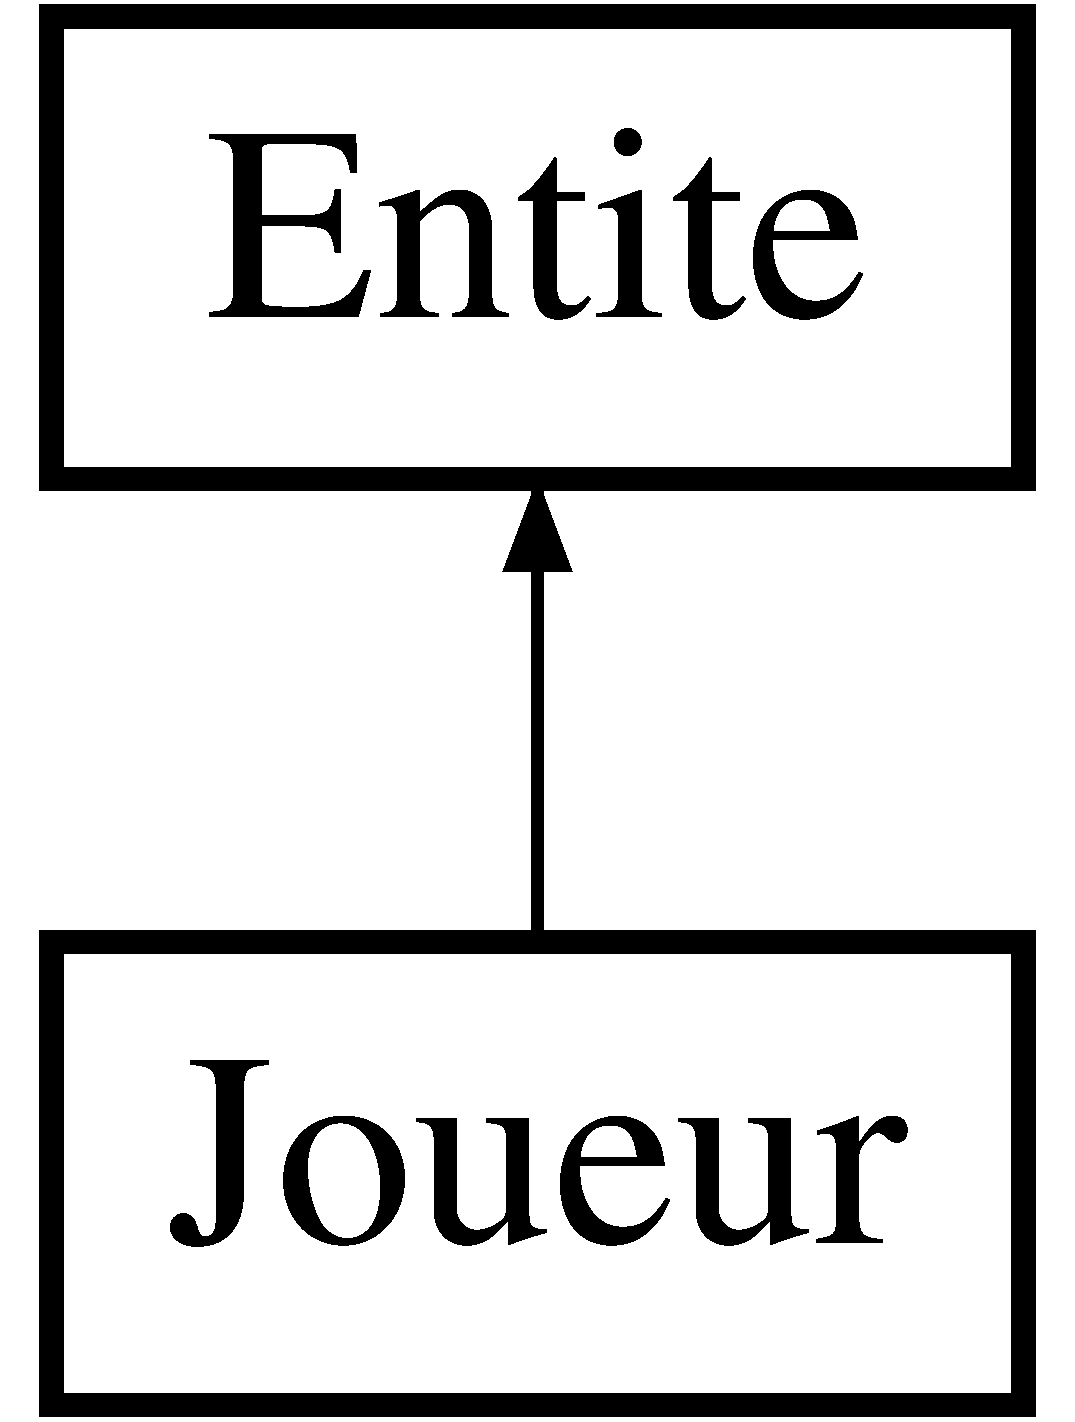
\includegraphics[height=2.000000cm]{class_joueur}
\end{center}
\end{figure}
\subsection*{Public Member Functions}
\begin{DoxyCompactItemize}
\item 
\mbox{\Hypertarget{class_joueur_affaf3cbb532de17e8e2308dd94041ca5}\label{class_joueur_affaf3cbb532de17e8e2308dd94041ca5}} 
sf\+::\+Vector2f {\bfseries deplacement} ()
\item 
\mbox{\Hypertarget{class_joueur_a30328b5202617be22da3a53d00a6feb4}\label{class_joueur_a30328b5202617be22da3a53d00a6feb4}} 
void {\bfseries collision\+Ennemi} (\mbox{\hyperlink{class_ennemi}{Ennemi}} ennemi)
\item 
\mbox{\Hypertarget{class_joueur_aafe639c272e0840a2fdab8f98883495f}\label{class_joueur_aafe639c272e0840a2fdab8f98883495f}} 
void \mbox{\hyperlink{class_joueur_aafe639c272e0840a2fdab8f98883495f}{collision\+Bordure}} (\mbox{\hyperlink{class_bordure}{Bordure}} bordure)
\begin{DoxyCompactList}\small\item\em Fonction g�rant la collision avec les ennemis. \end{DoxyCompactList}\item 
\mbox{\Hypertarget{class_joueur_a283dfffc2c544e5e1ec7bf8ba5f9eb86}\label{class_joueur_a283dfffc2c544e5e1ec7bf8ba5f9eb86}} 
void \mbox{\hyperlink{class_joueur_a283dfffc2c544e5e1ec7bf8ba5f9eb86}{joueur\+Repop\+Invincible}} (sf\+::\+Clock \mbox{\hyperlink{class_joueur_a44430a894e00f3e94c72af4e29cf862c}{clock}})
\begin{DoxyCompactList}\small\item\em Fonction g�rant la collision avec les bords de l\textquotesingle{}�cran. \end{DoxyCompactList}\item 
\mbox{\Hypertarget{class_joueur_a11311581a6d1c82dc8b6cc0944c45d66}\label{class_joueur_a11311581a6d1c82dc8b6cc0944c45d66}} 
void \mbox{\hyperlink{class_joueur_a11311581a6d1c82dc8b6cc0944c45d66}{joueur\+Normal\+Apres\+Invincible}} ()
\begin{DoxyCompactList}\small\item\em Fonction permettant de faire r�apparaitre le joueur � sa position initiale lorsqu\textquotesingle{}il est touch� et de le rendre invincible pendant quelques secondes. \end{DoxyCompactList}\item 
\mbox{\Hypertarget{class_joueur_aa898012c7e1be28dab380b66cfe80619}\label{class_joueur_aa898012c7e1be28dab380b66cfe80619}} 
void \mbox{\hyperlink{class_joueur_aa898012c7e1be28dab380b66cfe80619}{jaugecanon}} ()
\begin{DoxyCompactList}\small\item\em Le joueur redevient normal et vuln�rable. \end{DoxyCompactList}\end{DoxyCompactItemize}
\subsection*{Public Attributes}
\begin{DoxyCompactItemize}
\item 
\mbox{\Hypertarget{class_joueur_ab48403f63a4482a004f3ad4968868d2a}\label{class_joueur_ab48403f63a4482a004f3ad4968868d2a}} 
sf\+::\+Vector2f \mbox{\hyperlink{class_joueur_ab48403f63a4482a004f3ad4968868d2a}{joueur\+Position\+Precedente}}
\begin{DoxyCompactList}\small\item\em gestion de la jauge diminuant lors de l\textquotesingle{}utilisation du canon \end{DoxyCompactList}\item 
\mbox{\Hypertarget{class_joueur_abd5a7ad29404d19fdd7654ba246c7613}\label{class_joueur_abd5a7ad29404d19fdd7654ba246c7613}} 
sf\+::\+Texture \mbox{\hyperlink{class_joueur_abd5a7ad29404d19fdd7654ba246c7613}{texture}}
\begin{DoxyCompactList}\small\item\em position utilis�e lors des collisions avec les bords de l\textquotesingle{}�cran \end{DoxyCompactList}\item 
\mbox{\Hypertarget{class_joueur_a4a82216c7470860f2f3f8475ce6177ae}\label{class_joueur_a4a82216c7470860f2f3f8475ce6177ae}} 
sf\+::\+Rectangle\+Shape \mbox{\hyperlink{class_joueur_a4a82216c7470860f2f3f8475ce6177ae}{hit\+Box\+Joueur}}
\begin{DoxyCompactList}\small\item\em texture du joueur \end{DoxyCompactList}\item 
\mbox{\Hypertarget{class_joueur_aca8838903a5f779e69c7989a76bbe26a}\label{class_joueur_aca8838903a5f779e69c7989a76bbe26a}} 
sf\+::\+Rectangle\+Shape \mbox{\hyperlink{class_joueur_aca8838903a5f779e69c7989a76bbe26a}{forme\+Jauge\+Canon}}
\begin{DoxyCompactList}\small\item\em forme repr�sentant la hitbox du joueur \end{DoxyCompactList}\item 
\mbox{\Hypertarget{class_joueur_a7935eefd61dbbf420116236a7ba068fd}\label{class_joueur_a7935eefd61dbbf420116236a7ba068fd}} 
sf\+::\+Rectangle\+Shape \mbox{\hyperlink{class_joueur_a7935eefd61dbbf420116236a7ba068fd}{contour\+Jauge\+Canon}}
\begin{DoxyCompactList}\small\item\em forme repr�sentant la jauge du canon \end{DoxyCompactList}\item 
\mbox{\Hypertarget{class_joueur_a77d0ff40f510bbc57879ea2c415e3a50}\label{class_joueur_a77d0ff40f510bbc57879ea2c415e3a50}} 
float \mbox{\hyperlink{class_joueur_a77d0ff40f510bbc57879ea2c415e3a50}{vitesse}}
\begin{DoxyCompactList}\small\item\em bordure de la jauge du canon \end{DoxyCompactList}\item 
\mbox{\Hypertarget{class_joueur_a3c2aedb65e63a8e62ed6a4bda3b4cf27}\label{class_joueur_a3c2aedb65e63a8e62ed6a4bda3b4cf27}} 
int \mbox{\hyperlink{class_joueur_a3c2aedb65e63a8e62ed6a4bda3b4cf27}{pv}}
\begin{DoxyCompactList}\small\item\em vitesse du joueur \end{DoxyCompactList}\item 
\mbox{\Hypertarget{class_joueur_a7616d37e17b6894b61cb0090bafcc739}\label{class_joueur_a7616d37e17b6894b61cb0090bafcc739}} 
bool \mbox{\hyperlink{class_joueur_a7616d37e17b6894b61cb0090bafcc739}{invincible}}
\begin{DoxyCompactList}\small\item\em points de vie du joueur \end{DoxyCompactList}\item 
\mbox{\Hypertarget{class_joueur_ac373cdd21b69d52a960c7430125e41a3}\label{class_joueur_ac373cdd21b69d52a960c7430125e41a3}} 
bool \mbox{\hyperlink{class_joueur_ac373cdd21b69d52a960c7430125e41a3}{move}}
\begin{DoxyCompactList}\small\item\em �tat invincible ou non \end{DoxyCompactList}\item 
\mbox{\Hypertarget{class_joueur_a8c1f6a4f816388bd77e3a1002b102684}\label{class_joueur_a8c1f6a4f816388bd77e3a1002b102684}} 
bool \mbox{\hyperlink{class_joueur_a8c1f6a4f816388bd77e3a1002b102684}{temps\+Restart}}
\begin{DoxyCompactList}\small\item\em le joueur peut bouger ou non \end{DoxyCompactList}\item 
\mbox{\Hypertarget{class_joueur_a705a4994902943b4bf0b37b37db1a95c}\label{class_joueur_a705a4994902943b4bf0b37b37db1a95c}} 
bool {\bfseries boom}
\item 
\mbox{\Hypertarget{class_joueur_a8d0d4ed7dfb0a9cc20d3f0f328a7a852}\label{class_joueur_a8d0d4ed7dfb0a9cc20d3f0f328a7a852}} 
bool {\bfseries tir\+OK} = true
\item 
\mbox{\Hypertarget{class_joueur_a12525a5ca0c607ccf3403e5f8c3a1bda}\label{class_joueur_a12525a5ca0c607ccf3403e5f8c3a1bda}} 
bool \mbox{\hyperlink{class_joueur_a12525a5ca0c607ccf3403e5f8c3a1bda}{canon\+Actif}} = false
\begin{DoxyCompactList}\small\item\em le joueur peut tirer ou non \end{DoxyCompactList}\item 
\mbox{\Hypertarget{class_joueur_aedef76a29c76026dbb6b01a0884e05dc}\label{class_joueur_aedef76a29c76026dbb6b01a0884e05dc}} 
bool \mbox{\hyperlink{class_joueur_aedef76a29c76026dbb6b01a0884e05dc}{S\+FX}} = false
\begin{DoxyCompactList}\small\item\em permet de v�rifier si la touche d\textquotesingle{}activation du canon est enfonc�e ou pas \end{DoxyCompactList}\item 
\mbox{\Hypertarget{class_joueur_ae253373e58b6eb673ac4ae093bc3b366}\label{class_joueur_ae253373e58b6eb673ac4ae093bc3b366}} 
int \mbox{\hyperlink{class_joueur_ae253373e58b6eb673ac4ae093bc3b366}{i}} = 0
\begin{DoxyCompactList}\small\item\em activation des effets sonores \end{DoxyCompactList}\item 
\mbox{\Hypertarget{class_joueur_afc5f403f130bb3426dffca6a24d79538}\label{class_joueur_afc5f403f130bb3426dffca6a24d79538}} 
float \mbox{\hyperlink{class_joueur_afc5f403f130bb3426dffca6a24d79538}{valeur\+Jauge\+Canon}} = 100
\begin{DoxyCompactList}\small\item\em incr�menteur utilis� pour l\textquotesingle{}animation du joueur \end{DoxyCompactList}\item 
\mbox{\Hypertarget{class_joueur_a44430a894e00f3e94c72af4e29cf862c}\label{class_joueur_a44430a894e00f3e94c72af4e29cf862c}} 
sf\+::\+Clock \mbox{\hyperlink{class_joueur_a44430a894e00f3e94c72af4e29cf862c}{clock}}
\begin{DoxyCompactList}\small\item\em valeur de la jauge du canon \end{DoxyCompactList}\end{DoxyCompactItemize}


\subsection{Detailed Description}
Classe de cr�ation du joueur. 

The documentation for this class was generated from the following files\+:\begin{DoxyCompactItemize}
\item 
prog/Joueur.\+h\item 
prog/Joueur.\+cpp\end{DoxyCompactItemize}

\hypertarget{class_missile}{}\section{Missile Class Reference}
\label{class_missile}\index{Missile@{Missile}}


Projectiles du joueur (2 types, missile et canon)  




{\ttfamily \#include $<$Missile.\+h$>$}

Inheritance diagram for Missile\+:\begin{figure}[H]
\begin{center}
\leavevmode
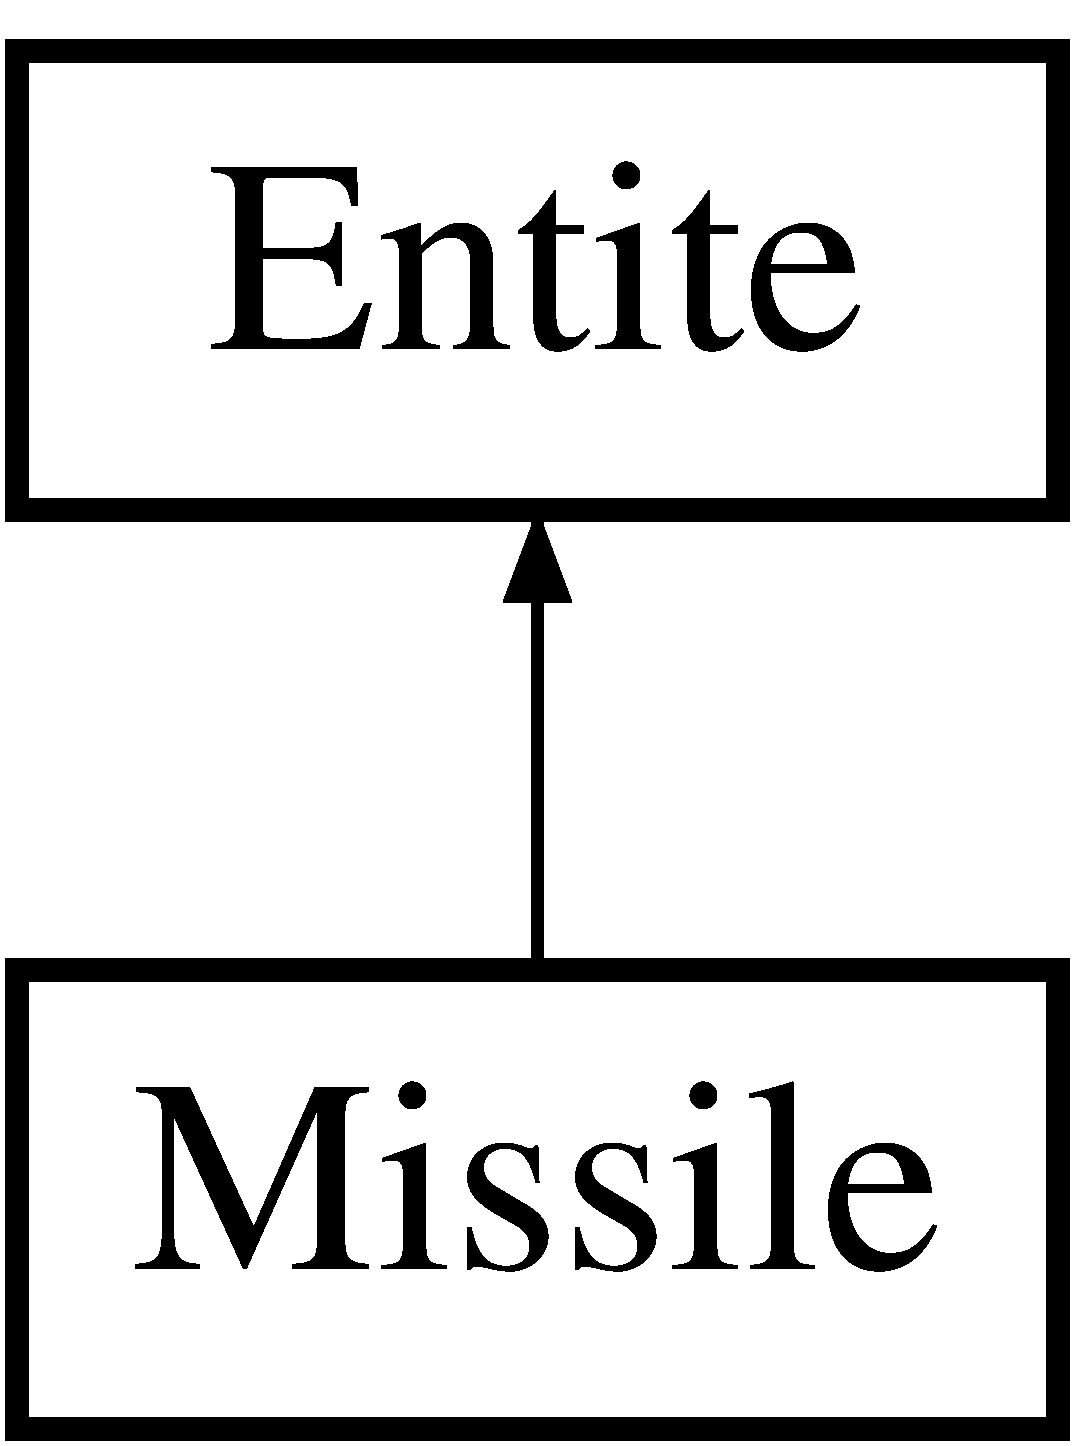
\includegraphics[height=2.000000cm]{class_missile}
\end{center}
\end{figure}
\subsection*{Additional Inherited Members}


\subsection{Detailed Description}
Projectiles du joueur (2 types, missile et canon) 

The documentation for this class was generated from the following files\+:\begin{DoxyCompactItemize}
\item 
prog/Missile.\+h\item 
prog/Missile.\+cpp\end{DoxyCompactItemize}

\hypertarget{class_missile_ennemi}{}\section{Missile\+Ennemi Class Reference}
\label{class_missile_ennemi}\index{Missile\+Ennemi@{Missile\+Ennemi}}


Classe de cr�ation des projectiles des ennemis.  




{\ttfamily \#include $<$Missile\+Ennemi.\+h$>$}

Inheritance diagram for Missile\+Ennemi\+:\begin{figure}[H]
\begin{center}
\leavevmode
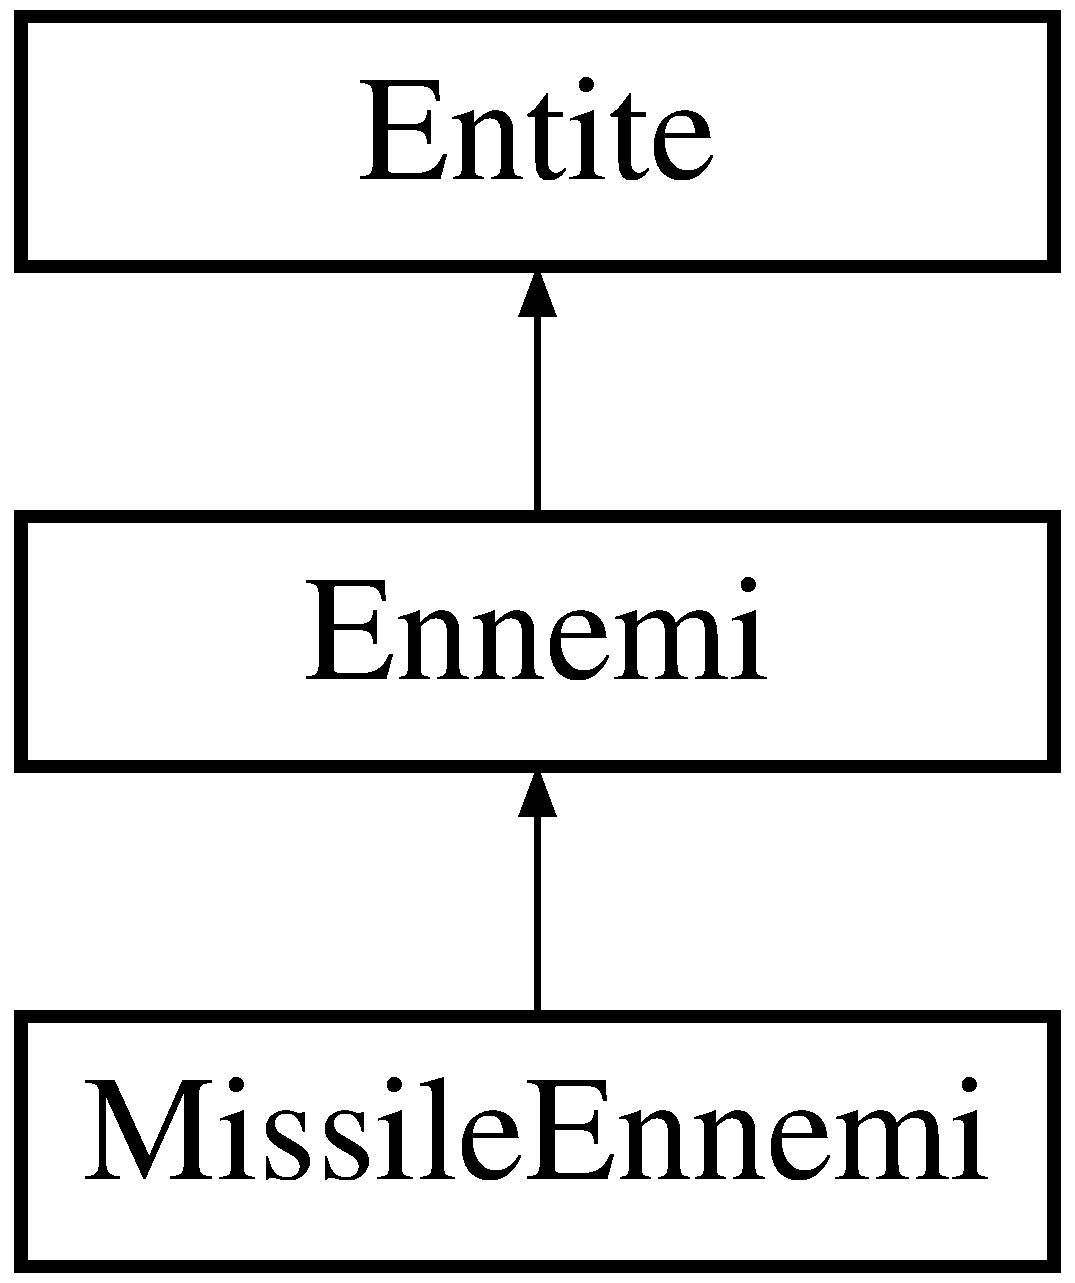
\includegraphics[height=3.000000cm]{class_missile_ennemi}
\end{center}
\end{figure}
\subsection*{Additional Inherited Members}


\subsection{Detailed Description}
Classe de cr�ation des projectiles des ennemis. 

The documentation for this class was generated from the following files\+:\begin{DoxyCompactItemize}
\item 
prog/Missile\+Ennemi.\+h\item 
prog/Missile\+Ennemi.\+cpp\end{DoxyCompactItemize}

\hypertarget{class_niveaux}{}\section{Niveaux Class Reference}
\label{class_niveaux}\index{Niveaux@{Niveaux}}


Classe de cr�ation des niveaux faisant office d\textquotesingle{}�diteur de niveaux.  




{\ttfamily \#include $<$Niveaux.\+h$>$}

\subsection*{Public Member Functions}
\begin{DoxyCompactItemize}
\item 
\mbox{\Hypertarget{class_niveaux_a9cc426bdc08db384dfa02c69bb6c6f96}\label{class_niveaux_a9cc426bdc08db384dfa02c69bb6c6f96}} 
void \mbox{\hyperlink{class_niveaux_a9cc426bdc08db384dfa02c69bb6c6f96}{niveau1}} ()
\begin{DoxyCompactList}\small\item\em C\textquotesingle{}est ici que sont cr��s les diff�rents niveaux. \end{DoxyCompactList}\item 
\mbox{\Hypertarget{class_niveaux_a02e17b5525c5738e0b7317f3f4d04ad1}\label{class_niveaux_a02e17b5525c5738e0b7317f3f4d04ad1}} 
void \mbox{\hyperlink{class_niveaux_a02e17b5525c5738e0b7317f3f4d04ad1}{niveau2}} ()
\begin{DoxyCompactList}\small\item\em M�thode contenant toutes les donn�es du niveau 1. \end{DoxyCompactList}\item 
\mbox{\Hypertarget{class_niveaux_ab2b835ee8f509329ca8f5d83108fb2a8}\label{class_niveaux_ab2b835ee8f509329ca8f5d83108fb2a8}} 
void \mbox{\hyperlink{class_niveaux_ab2b835ee8f509329ca8f5d83108fb2a8}{niveau3}} ()
\begin{DoxyCompactList}\small\item\em M�thode contenant toutes les donn�es du niveau 2. \end{DoxyCompactList}\item 
\mbox{\Hypertarget{class_niveaux_a25b5210552a2500852e36cf79058537e}\label{class_niveaux_a25b5210552a2500852e36cf79058537e}} 
void \mbox{\hyperlink{class_niveaux_a25b5210552a2500852e36cf79058537e}{niveau4}} ()
\begin{DoxyCompactList}\small\item\em M�thode contenant toutes les donn�es du niveau 3. \end{DoxyCompactList}\item 
\mbox{\Hypertarget{class_niveaux_a28e3ac0fd958550e38bd9784f91b4064}\label{class_niveaux_a28e3ac0fd958550e38bd9784f91b4064}} 
void \mbox{\hyperlink{class_niveaux_a28e3ac0fd958550e38bd9784f91b4064}{niveau\+Test}} ()
\begin{DoxyCompactList}\small\item\em M�thode contenant toutes les donn�es du niveau 4. \end{DoxyCompactList}\item 
\mbox{\Hypertarget{class_niveaux_a4c70e2ed5a72255b274a4a8f8d032f7a}\label{class_niveaux_a4c70e2ed5a72255b274a4a8f8d032f7a}} 
void {\bfseries gestion\+Vecteur\+Ennemis\+Et\+Missiles\+Ennemis} ()
\item 
int \mbox{\hyperlink{class_niveaux_af01fdf0f42d54fea61f299a5875b16d3}{ennemi\+Pop}} (unsigned int vitesse)
\begin{DoxyCompactList}\small\item\em vitesse d\textquotesingle{}apparition des ennemis de type boss \end{DoxyCompactList}\item 
int \mbox{\hyperlink{class_niveaux_abd64ac2e8891cfb204ebd5e433ff94b6}{aleatoire}} ()
\begin{DoxyCompactList}\small\item\em Vector contenant les diff�rents ennemis. \end{DoxyCompactList}\item 
void \mbox{\hyperlink{class_niveaux_af01fef3a80ba9ff2083a06fc2e6b0abd}{lancement\+Ennemis1}} (float debut, float fin, int vitesse\+Apparition, int x, int y, float vitesseX, float vitesseY)
\begin{DoxyCompactList}\small\item\em Cr�ation d\textquotesingle{}un objet \mbox{\hyperlink{class_joueur}{Joueur}}. \end{DoxyCompactList}\item 
\mbox{\Hypertarget{class_niveaux_a106d71ceea76ee60ca90c47963442b9b}\label{class_niveaux_a106d71ceea76ee60ca90c47963442b9b}} 
void {\bfseries lancement\+Ennemis12} (float debut, float fin, int vitesse\+Apparition, int x, int y, float vitesseX, float vitesseY)
\item 
\mbox{\Hypertarget{class_niveaux_acd52f679ab3d0e504a8c5168275efcd2}\label{class_niveaux_acd52f679ab3d0e504a8c5168275efcd2}} 
void {\bfseries lancement\+Ennemis2} (float debut, float fin, int vitesse\+Apparition, int x, int y, float vitesseX, float vitesseY)
\item 
\mbox{\Hypertarget{class_niveaux_a06828646654b91d9feab64227753bfb4}\label{class_niveaux_a06828646654b91d9feab64227753bfb4}} 
void {\bfseries lancement\+Ennemis3} (float debut, float fin, int vitesse\+Apparition, int x, int y, float vitesseX, float vitesseY)
\item 
\mbox{\Hypertarget{class_niveaux_af23d1e7d05ffd22dd6c283af89b74d2a}\label{class_niveaux_af23d1e7d05ffd22dd6c283af89b74d2a}} 
void \mbox{\hyperlink{class_niveaux_af23d1e7d05ffd22dd6c283af89b74d2a}{rotation\+Ennemis}} ()
\begin{DoxyCompactList}\small\item\em Cette fonction permet de g�rer l\textquotesingle{}orientation de l\textquotesingle{}ennemi dans le sens de son d�placement. \end{DoxyCompactList}\item 
sf\+::\+Vector2f \mbox{\hyperlink{class_niveaux_a4a42871f41dc2124a8bf272bc877381e}{tete\+Chercheuse}} (\mbox{\hyperlink{class_joueur}{Joueur}} \mbox{\hyperlink{class_niveaux_a5b99cb21e16562ea3e65f89fa6e35372}{joueur}}, \mbox{\hyperlink{class_ennemi}{Ennemi}} ennemi, float vitesse, float x\+Rand)
\item 
\mbox{\Hypertarget{class_niveaux_a92efdde72dceef45f8bf6b1e3f393a58}\label{class_niveaux_a92efdde72dceef45f8bf6b1e3f393a58}} 
sf\+::\+Vector2f \mbox{\hyperlink{class_niveaux_a92efdde72dceef45f8bf6b1e3f393a58}{tete\+Chercheuse}} (\mbox{\hyperlink{class_joueur}{Joueur}} \mbox{\hyperlink{class_niveaux_a5b99cb21e16562ea3e65f89fa6e35372}{joueur}}, int pos, float vitesse)
\begin{DoxyCompactList}\small\item\em Version surcharg�e avec un argument en moins afin de l\textquotesingle{}utiliser pour d�placer un ennemi vers la position du joueur. \end{DoxyCompactList}\item 
\mbox{\Hypertarget{class_niveaux_a1390969eae72324ee7f707ecbf64b3fc}\label{class_niveaux_a1390969eae72324ee7f707ecbf64b3fc}} 
sf\+::\+Vector2f \mbox{\hyperlink{class_niveaux_a1390969eae72324ee7f707ecbf64b3fc}{spirale}} (float vitesse\+Rotation, float vitesse\+Deplacement)
\begin{DoxyCompactList}\small\item\em Pattern de tir en forme de spirale. \end{DoxyCompactList}\item 
\mbox{\Hypertarget{class_niveaux_aac23502d5ea1d6bd7b645b321b5271e2}\label{class_niveaux_aac23502d5ea1d6bd7b645b321b5271e2}} 
sf\+::\+Vector2f \mbox{\hyperlink{class_niveaux_aac23502d5ea1d6bd7b645b321b5271e2}{reverse\+Spirale}} (float vitesse\+Rotation, float vitesse\+Deplacement)
\begin{DoxyCompactList}\small\item\em Pattern en spirale invers�e \end{DoxyCompactList}\item 
\mbox{\Hypertarget{class_niveaux_a307a834f4fa05bf1c727b2153881d66b}\label{class_niveaux_a307a834f4fa05bf1c727b2153881d66b}} 
bool \mbox{\hyperlink{class_niveaux_a307a834f4fa05bf1c727b2153881d66b}{tirY}} (\mbox{\hyperlink{class_ennemi}{Ennemi}} ennemi, int debut, int fin)
\begin{DoxyCompactList}\small\item\em L\textquotesingle{}ennemi se met � tirer � la position \char`\"{}d�but\char`\"{} et cesse � la position \char`\"{}fin\char`\"{} (en onrdonn�e) \end{DoxyCompactList}\item 
\mbox{\Hypertarget{class_niveaux_a0bebae4c6f6b1cb3b772b9e2f79d0d00}\label{class_niveaux_a0bebae4c6f6b1cb3b772b9e2f79d0d00}} 
bool \mbox{\hyperlink{class_niveaux_a0bebae4c6f6b1cb3b772b9e2f79d0d00}{tirX}} (\mbox{\hyperlink{class_ennemi}{Ennemi}} ennemi, int debut, int fin)
\begin{DoxyCompactList}\small\item\em L\textquotesingle{}ennemi se met � tirer � la position \char`\"{}d�but\char`\"{} et cesse � la position \char`\"{}fin\char`\"{} (en abscisse) \end{DoxyCompactList}\end{DoxyCompactItemize}
\subsection*{Public Attributes}
\begin{DoxyCompactItemize}
\item 
bool \mbox{\hyperlink{class_niveaux_ae819d9af466367e01744cd5d848b5482}{shoot1}} = false
\begin{DoxyCompactList}\small\item\em fonction permettant de placer les ennemis et les projectiles ennemis dans un vecteur \end{DoxyCompactList}\item 
\mbox{\Hypertarget{class_niveaux_ab296ae58a3c1785e695850096aff095d}\label{class_niveaux_ab296ae58a3c1785e695850096aff095d}} 
bool \mbox{\hyperlink{class_niveaux_ab296ae58a3c1785e695850096aff095d}{shoot12}} = false
\begin{DoxyCompactList}\small\item\em Lancement des objets ennemi1. \end{DoxyCompactList}\item 
\mbox{\Hypertarget{class_niveaux_accc6a92a050730ee2ee28b50da765946}\label{class_niveaux_accc6a92a050730ee2ee28b50da765946}} 
bool \mbox{\hyperlink{class_niveaux_accc6a92a050730ee2ee28b50da765946}{shoot2}} = false
\begin{DoxyCompactList}\small\item\em Lancement des objets ennemi12. \end{DoxyCompactList}\item 
\mbox{\Hypertarget{class_niveaux_a7244489a9a5e378202d8c9dcacb3b81a}\label{class_niveaux_a7244489a9a5e378202d8c9dcacb3b81a}} 
bool \mbox{\hyperlink{class_niveaux_a7244489a9a5e378202d8c9dcacb3b81a}{shoot3}} = false
\begin{DoxyCompactList}\small\item\em Lancement des objets ennemi2. \end{DoxyCompactList}\item 
\mbox{\Hypertarget{class_niveaux_ad96e2b7a2aa6b317e238f0569d4a34ba}\label{class_niveaux_ad96e2b7a2aa6b317e238f0569d4a34ba}} 
bool \mbox{\hyperlink{class_niveaux_ad96e2b7a2aa6b317e238f0569d4a34ba}{shoot\+Boss}} = false
\begin{DoxyCompactList}\small\item\em Lancement des objets ennemi3. \end{DoxyCompactList}\item 
\mbox{\Hypertarget{class_niveaux_ae17183082440ab27c83bc6aa670f645e}\label{class_niveaux_ae17183082440ab27c83bc6aa670f645e}} 
bool \mbox{\hyperlink{class_niveaux_ae17183082440ab27c83bc6aa670f645e}{shoot\+Boss\+Final}} = false
\begin{DoxyCompactList}\small\item\em Lancement du boss 1. \end{DoxyCompactList}\item 
\mbox{\Hypertarget{class_niveaux_a1330f8179bc2a3ecb8d4e0bf9ca76aaa}\label{class_niveaux_a1330f8179bc2a3ecb8d4e0bf9ca76aaa}} 
bool \mbox{\hyperlink{class_niveaux_a1330f8179bc2a3ecb8d4e0bf9ca76aaa}{fini}} = false
\begin{DoxyCompactList}\small\item\em Lancement du boss final. \end{DoxyCompactList}\item 
\mbox{\Hypertarget{class_niveaux_a66ac0f6a0dae223d1fd9dbe52e80a537}\label{class_niveaux_a66ac0f6a0dae223d1fd9dbe52e80a537}} 
bool \mbox{\hyperlink{class_niveaux_a66ac0f6a0dae223d1fd9dbe52e80a537}{fin\+Du\+Jeu}} = false
\begin{DoxyCompactList}\small\item\em Lorsqu\textquotesingle{}il est T\+R\+UE, le niveau est termin�. Sa valeur est test�e � la ligne 424 de la classe Game.\+cpp et permet de passer � l\textquotesingle{}�cran \char`\"{}\+M\+I\+S\+S\+I\+O\+N\+A\+C\+C\+O\+M\+P\+L\+I\+E\char`\"{}. \end{DoxyCompactList}\item 
\mbox{\Hypertarget{class_niveaux_a3ebda11eb8c60b0627a4cacc682cf325}\label{class_niveaux_a3ebda11eb8c60b0627a4cacc682cf325}} 
bool \mbox{\hyperlink{class_niveaux_a3ebda11eb8c60b0627a4cacc682cf325}{go}} = false
\begin{DoxyCompactList}\small\item\em Lorsqu\textquotesingle{}il est T\+R\+EU, permet de passer au �cran de fin du jeu. \end{DoxyCompactList}\item 
\mbox{\Hypertarget{class_niveaux_af6c482aa96abde442494ad353a456f90}\label{class_niveaux_af6c482aa96abde442494ad353a456f90}} 
bool \mbox{\hyperlink{class_niveaux_af6c482aa96abde442494ad353a456f90}{boss\+Go}} = false
\begin{DoxyCompactList}\small\item\em Il arrive qu\textquotesingle{}un ennemi \char`\"{}bloque\char`\"{} l\textquotesingle{}action tant que ses PV$>$0. Ce bool�en permet de relancer l\textquotesingle{}action une fois les PV=0. \end{DoxyCompactList}\item 
\mbox{\Hypertarget{class_niveaux_a310e91860a7fb1047742b4654c231fe0}\label{class_niveaux_a310e91860a7fb1047742b4654c231fe0}} 
bool \mbox{\hyperlink{class_niveaux_a310e91860a7fb1047742b4654c231fe0}{boss\+Pattern}} = false
\begin{DoxyCompactList}\small\item\em Utilis� pour lancer l\textquotesingle{}action du boss. \end{DoxyCompactList}\item 
\mbox{\Hypertarget{class_niveaux_ae987b39fd8bc72779775cc2daa13be72}\label{class_niveaux_ae987b39fd8bc72779775cc2daa13be72}} 
bool \mbox{\hyperlink{class_niveaux_ae987b39fd8bc72779775cc2daa13be72}{missile2\+Actif}} = true
\begin{DoxyCompactList}\small\item\em quand il est T\+R\+UE, permet de lancer le pattern droite/gauche du boss \end{DoxyCompactList}\item 
\mbox{\Hypertarget{class_niveaux_a753971022f595dd0c3ebb470b9aa9eba}\label{class_niveaux_a753971022f595dd0c3ebb470b9aa9eba}} 
sf\+::\+Clock \mbox{\hyperlink{class_niveaux_a753971022f595dd0c3ebb470b9aa9eba}{clock1}}
\begin{DoxyCompactList}\small\item\em Permet d\textquotesingle{}activer le deuxi�me vector de projectiles ennemis. \end{DoxyCompactList}\item 
sf\+::\+Clock \mbox{\hyperlink{class_niveaux_a4a93683a35a90181218f8858a883a93a}{vitesse\+Ennemi\+Pop1}}
\begin{DoxyCompactList}\small\item\em Ces clocks permettent de g�rer la vitesse � laquelle les ennemis/boss sont plac� dans le vecteur d\textquotesingle{}ennemis. \end{DoxyCompactList}\item 
\mbox{\Hypertarget{class_niveaux_acea936f3ad9dd6cbb17818ca75d43bdf}\label{class_niveaux_acea936f3ad9dd6cbb17818ca75d43bdf}} 
sf\+::\+Clock \mbox{\hyperlink{class_niveaux_acea936f3ad9dd6cbb17818ca75d43bdf}{vitesse\+Ennemi\+Pop2}}
\begin{DoxyCompactList}\small\item\em vitesse de mise en vecteur des ennemis de type 1 \end{DoxyCompactList}\item 
\mbox{\Hypertarget{class_niveaux_a01d964627863fce4c63396a53a3803d5}\label{class_niveaux_a01d964627863fce4c63396a53a3803d5}} 
sf\+::\+Clock \mbox{\hyperlink{class_niveaux_a01d964627863fce4c63396a53a3803d5}{vitesse\+Ennemi\+Pop3}}
\begin{DoxyCompactList}\small\item\em vitesse de mise en vecteur des ennemis de type 2 \end{DoxyCompactList}\item 
\mbox{\Hypertarget{class_niveaux_a9735f68c6435670e148f131a1a293082}\label{class_niveaux_a9735f68c6435670e148f131a1a293082}} 
sf\+::\+Clock \mbox{\hyperlink{class_niveaux_a9735f68c6435670e148f131a1a293082}{vitesse\+Boss\+Pop}}
\begin{DoxyCompactList}\small\item\em vitesse de mise en vecteur des ennemis de type 3 \end{DoxyCompactList}\item 
unsigned int \mbox{\hyperlink{class_niveaux_aaa933f742de563656272d55922248d25}{vitesse\+Apparition1}}
\begin{DoxyCompactList}\small\item\em Utilis�es dans les fonctions \char`\"{}lancement\+Ennemis\char`\"{}, permettent de g�rer � quelle vitesse les ennemis apparaissent. \end{DoxyCompactList}\item 
\mbox{\Hypertarget{class_niveaux_a9f51f17b5734f335bd82f3e6a641d4b0}\label{class_niveaux_a9f51f17b5734f335bd82f3e6a641d4b0}} 
unsigned int \mbox{\hyperlink{class_niveaux_a9f51f17b5734f335bd82f3e6a641d4b0}{vitesse\+Apparition12}}
\begin{DoxyCompactList}\small\item\em vitesse d\textquotesingle{}apparition des ennemis de type 1 \end{DoxyCompactList}\item 
\mbox{\Hypertarget{class_niveaux_a5c3a73252693b4ebcec5d34ca9c548fa}\label{class_niveaux_a5c3a73252693b4ebcec5d34ca9c548fa}} 
unsigned int \mbox{\hyperlink{class_niveaux_a5c3a73252693b4ebcec5d34ca9c548fa}{vitesse\+Apparition2}}
\begin{DoxyCompactList}\small\item\em vitesse d\textquotesingle{}apparition des ennemis de type 12 \end{DoxyCompactList}\item 
\mbox{\Hypertarget{class_niveaux_a677d8748e518d63bc5eabc72ea1534e4}\label{class_niveaux_a677d8748e518d63bc5eabc72ea1534e4}} 
unsigned int \mbox{\hyperlink{class_niveaux_a677d8748e518d63bc5eabc72ea1534e4}{vitesse\+Apparition3}}
\begin{DoxyCompactList}\small\item\em vitesse d\textquotesingle{}apparition des ennemis de type 2 \end{DoxyCompactList}\item 
\mbox{\Hypertarget{class_niveaux_a1c4457048368416deb18ee2e60e72d2d}\label{class_niveaux_a1c4457048368416deb18ee2e60e72d2d}} 
unsigned int \mbox{\hyperlink{class_niveaux_a1c4457048368416deb18ee2e60e72d2d}{vitesse\+Apparition\+Boss}} = 10
\begin{DoxyCompactList}\small\item\em vitesse d\textquotesingle{}apparition des ennemis de type 3 \end{DoxyCompactList}\item 
\mbox{\Hypertarget{class_niveaux_a9f8a87aaddd8d4d0f74a276603fee4e6}\label{class_niveaux_a9f8a87aaddd8d4d0f74a276603fee4e6}} 
int {\bfseries app} = 30
\item 
\mbox{\Hypertarget{class_niveaux_a5434fbbbeaec027cad99bd5fbc0c61b7}\label{class_niveaux_a5434fbbbeaec027cad99bd5fbc0c61b7}} 
float \mbox{\hyperlink{class_niveaux_a5434fbbbeaec027cad99bd5fbc0c61b7}{vit}} = 12
\begin{DoxyCompactList}\small\item\em Utilis�e uniquement dans le niveau 3 pour g�rer le nombre d\textquotesingle{}ennemi d\textquotesingle{}une vague d\textquotesingle{}ennemis. \end{DoxyCompactList}\item 
\mbox{\hyperlink{class_ennemi1}{Ennemi1}} \mbox{\hyperlink{class_niveaux_ac8e66f8f91918ea9042cc5b6ae99f79f}{ennemi1}}
\begin{DoxyCompactList}\small\item\em Utilis�e uniquement dans le niveau 3 pour g�rer la vitesse d\textquotesingle{}apparition d\textquotesingle{}une vague d\textquotesingle{}ennemis. \end{DoxyCompactList}\item 
\mbox{\Hypertarget{class_niveaux_a6039ce685c6a188a36223e9f151ef438}\label{class_niveaux_a6039ce685c6a188a36223e9f151ef438}} 
\mbox{\hyperlink{class_ennemi1}{Ennemi1}} \mbox{\hyperlink{class_niveaux_a6039ce685c6a188a36223e9f151ef438}{ennemi12}}
\begin{DoxyCompactList}\small\item\em \mbox{\hyperlink{class_ennemi}{Ennemi}} de type 1. \end{DoxyCompactList}\item 
\mbox{\Hypertarget{class_niveaux_ae84ebb52117124dfe659f509076d4160}\label{class_niveaux_ae84ebb52117124dfe659f509076d4160}} 
\mbox{\hyperlink{class_ennemi2}{Ennemi2}} \mbox{\hyperlink{class_niveaux_ae84ebb52117124dfe659f509076d4160}{ennemi2}}
\begin{DoxyCompactList}\small\item\em \mbox{\hyperlink{class_ennemi}{Ennemi}} de type 12. \end{DoxyCompactList}\item 
\mbox{\Hypertarget{class_niveaux_a9adac325205adefd1501442f04829c7d}\label{class_niveaux_a9adac325205adefd1501442f04829c7d}} 
\mbox{\hyperlink{class_ennemi3}{Ennemi3}} \mbox{\hyperlink{class_niveaux_a9adac325205adefd1501442f04829c7d}{ennemi3}}
\begin{DoxyCompactList}\small\item\em \mbox{\hyperlink{class_ennemi}{Ennemi}} de type 2. \end{DoxyCompactList}\item 
\mbox{\Hypertarget{class_niveaux_aaa9a444f519d3b6257981d56c1b1267b}\label{class_niveaux_aaa9a444f519d3b6257981d56c1b1267b}} 
\mbox{\hyperlink{class_ennemi_boss}{Ennemi\+Boss}} \mbox{\hyperlink{class_niveaux_aaa9a444f519d3b6257981d56c1b1267b}{ennemi\+Boss}}
\begin{DoxyCompactList}\small\item\em \mbox{\hyperlink{class_ennemi}{Ennemi}} de type 3. \end{DoxyCompactList}\item 
\mbox{\Hypertarget{class_niveaux_afa208fdc622d37fc159924c5adf6b673}\label{class_niveaux_afa208fdc622d37fc159924c5adf6b673}} 
\mbox{\hyperlink{class_ennemi_boss}{Ennemi\+Boss}} \mbox{\hyperlink{class_niveaux_afa208fdc622d37fc159924c5adf6b673}{ennemi\+Boss\+Final}}
\begin{DoxyCompactList}\small\item\em Mini\+Boss du niveau 2. \end{DoxyCompactList}\item 
\mbox{\Hypertarget{class_niveaux_a0325043d76141629469469297fe00fca}\label{class_niveaux_a0325043d76141629469469297fe00fca}} 
std\+::vector$<$ \mbox{\hyperlink{class_ennemi}{Ennemi}} $>$ \mbox{\hyperlink{class_niveaux_a0325043d76141629469469297fe00fca}{ennemis}}
\begin{DoxyCompactList}\small\item\em Boss final. \end{DoxyCompactList}\item 
\mbox{\hyperlink{class_missile_ennemi}{Missile\+Ennemi}} \mbox{\hyperlink{class_niveaux_a47b36d93f889bd74a68a61ef1ac2c83d}{missile\+Ennemi}}
\item 
\mbox{\Hypertarget{class_niveaux_a5b1e8bdf82aef2f91f662d11d97b541f}\label{class_niveaux_a5b1e8bdf82aef2f91f662d11d97b541f}} 
\mbox{\hyperlink{class_missile_ennemi}{Missile\+Ennemi}} \mbox{\hyperlink{class_niveaux_a5b1e8bdf82aef2f91f662d11d97b541f}{missile\+Ennemi2}}
\begin{DoxyCompactList}\small\item\em Projectile ennemi 1. \end{DoxyCompactList}\item 
\mbox{\Hypertarget{class_niveaux_a11282a4434cac30a2189bcf5b005919d}\label{class_niveaux_a11282a4434cac30a2189bcf5b005919d}} 
std\+::vector$<$ \mbox{\hyperlink{class_ennemi}{Ennemi}} $>$ \mbox{\hyperlink{class_niveaux_a11282a4434cac30a2189bcf5b005919d}{vect\+Missile\+Ennemi}}
\begin{DoxyCompactList}\small\item\em Projectile ennemi 2. \end{DoxyCompactList}\item 
\mbox{\Hypertarget{class_niveaux_a6eada6e6f1fa1d2bc70c5d9d4f830437}\label{class_niveaux_a6eada6e6f1fa1d2bc70c5d9d4f830437}} 
float \mbox{\hyperlink{class_niveaux_a6eada6e6f1fa1d2bc70c5d9d4f830437}{angle}} = 0
\begin{DoxyCompactList}\small\item\em Vector contenant les projectiles ennemis. \end{DoxyCompactList}\item 
\mbox{\Hypertarget{class_niveaux_a99ed8ace369a3148d441f79efcd25011}\label{class_niveaux_a99ed8ace369a3148d441f79efcd25011}} 
float \mbox{\hyperlink{class_niveaux_a99ed8ace369a3148d441f79efcd25011}{angle2}} = 0
\begin{DoxyCompactList}\small\item\em Permet de faire varier l\textquotesingle{}angle de tir des ennemis, utilis� dans la fonction tir\+En\+Spirale. \end{DoxyCompactList}\item 
\mbox{\Hypertarget{class_niveaux_a12805d80b46378ccfa7198cbb567f8c7}\label{class_niveaux_a12805d80b46378ccfa7198cbb567f8c7}} 
int \mbox{\hyperlink{class_niveaux_a12805d80b46378ccfa7198cbb567f8c7}{vitesse\+Missile}} = 0
\begin{DoxyCompactList}\small\item\em Idem qu\textquotesingle{}angle mais pour les missile\+Ennemi2. \end{DoxyCompactList}\item 
\mbox{\Hypertarget{class_niveaux_ac8ba126c2d2ac1db1dc9ecd0e0fc0466}\label{class_niveaux_ac8ba126c2d2ac1db1dc9ecd0e0fc0466}} 
int \mbox{\hyperlink{class_niveaux_ac8ba126c2d2ac1db1dc9ecd0e0fc0466}{vitesse\+Missile2}} = 0
\begin{DoxyCompactList}\small\item\em Vitesse des projectiles ennemis. \end{DoxyCompactList}\item 
\mbox{\Hypertarget{class_niveaux_a5b99cb21e16562ea3e65f89fa6e35372}\label{class_niveaux_a5b99cb21e16562ea3e65f89fa6e35372}} 
\mbox{\hyperlink{class_joueur}{Joueur}} \mbox{\hyperlink{class_niveaux_a5b99cb21e16562ea3e65f89fa6e35372}{joueur}}
\begin{DoxyCompactList}\small\item\em Idem que vitesse\+Missile mais pour les missile\+Ennemi2. \end{DoxyCompactList}\end{DoxyCompactItemize}


\subsection{Detailed Description}
Classe de cr�ation des niveaux faisant office d\textquotesingle{}�diteur de niveaux. 

\subsection{Member Function Documentation}
\mbox{\Hypertarget{class_niveaux_abd64ac2e8891cfb204ebd5e433ff94b6}\label{class_niveaux_abd64ac2e8891cfb204ebd5e433ff94b6}} 
\index{Niveaux@{Niveaux}!aleatoire@{aleatoire}}
\index{aleatoire@{aleatoire}!Niveaux@{Niveaux}}
\subsubsection{\texorpdfstring{aleatoire()}{aleatoire()}}
{\footnotesize\ttfamily int Niveaux\+::aleatoire (\begin{DoxyParamCaption}{ }\end{DoxyParamCaption})\hspace{0.3cm}{\ttfamily [inline]}}



Vector contenant les diff�rents ennemis. 

P\+O\+S\+I\+T\+I\+ON Fonction g�n�rant une valeur al�atoire entre 0 et la largeur de l\textquotesingle{}�cran \mbox{\Hypertarget{class_niveaux_af01fdf0f42d54fea61f299a5875b16d3}\label{class_niveaux_af01fdf0f42d54fea61f299a5875b16d3}} 
\index{Niveaux@{Niveaux}!ennemi\+Pop@{ennemi\+Pop}}
\index{ennemi\+Pop@{ennemi\+Pop}!Niveaux@{Niveaux}}
\subsubsection{\texorpdfstring{ennemi\+Pop()}{ennemiPop()}}
{\footnotesize\ttfamily int Niveaux\+::ennemi\+Pop (\begin{DoxyParamCaption}\item[{unsigned int}]{vitesse }\end{DoxyParamCaption})\hspace{0.3cm}{\ttfamily [inline]}}



vitesse d\textquotesingle{}apparition des ennemis de type boss 

Fonction utilisant la vitesse\+Apparition, permet de convertir la vitesse\+Apparition pour faciliter la gestion par l\textquotesingle{}utilisateur \mbox{\Hypertarget{class_niveaux_af01fef3a80ba9ff2083a06fc2e6b0abd}\label{class_niveaux_af01fef3a80ba9ff2083a06fc2e6b0abd}} 
\index{Niveaux@{Niveaux}!lancement\+Ennemis1@{lancement\+Ennemis1}}
\index{lancement\+Ennemis1@{lancement\+Ennemis1}!Niveaux@{Niveaux}}
\subsubsection{\texorpdfstring{lancement\+Ennemis1()}{lancementEnnemis1()}}
{\footnotesize\ttfamily void Niveaux\+::lancement\+Ennemis1 (\begin{DoxyParamCaption}\item[{float}]{debut,  }\item[{float}]{fin,  }\item[{int}]{vitesse\+Apparition,  }\item[{int}]{x,  }\item[{int}]{y,  }\item[{float}]{vitesseX,  }\item[{float}]{vitesseY }\end{DoxyParamCaption})\hspace{0.3cm}{\ttfamily [inline]}}



Cr�ation d\textquotesingle{}un objet \mbox{\hyperlink{class_joueur}{Joueur}}. 

L\+A\+N\+C\+E\+M\+E\+NT D\+ES E\+N\+N\+E\+M\+IS Ces fonctions permettent de nettement faciliter la mani�re de lancer les ennemis, voir leur param�tres \mbox{\Hypertarget{class_niveaux_a4a42871f41dc2124a8bf272bc877381e}\label{class_niveaux_a4a42871f41dc2124a8bf272bc877381e}} 
\index{Niveaux@{Niveaux}!tete\+Chercheuse@{tete\+Chercheuse}}
\index{tete\+Chercheuse@{tete\+Chercheuse}!Niveaux@{Niveaux}}
\subsubsection{\texorpdfstring{tete\+Chercheuse()}{teteChercheuse()}}
{\footnotesize\ttfamily sf\+::\+Vector2f Niveaux\+::tete\+Chercheuse (\begin{DoxyParamCaption}\item[{\mbox{\hyperlink{class_joueur}{Joueur}}}]{joueur,  }\item[{\mbox{\hyperlink{class_ennemi}{Ennemi}}}]{ennemi,  }\item[{float}]{vitesse,  }\item[{float}]{x\+Rand }\end{DoxyParamCaption})\hspace{0.3cm}{\ttfamily [inline]}}

T\+IR D\+ES E\+N\+N\+E\+M\+IS Pattern t�te chercheuse, d�place un projectile ennemi depuis la position de l\textquotesingle{}ennemi vers la position du joueur (r�cup�r�e au moment o� le projectile est tir�) 

\subsection{Member Data Documentation}
\mbox{\Hypertarget{class_niveaux_ac8e66f8f91918ea9042cc5b6ae99f79f}\label{class_niveaux_ac8e66f8f91918ea9042cc5b6ae99f79f}} 
\index{Niveaux@{Niveaux}!ennemi1@{ennemi1}}
\index{ennemi1@{ennemi1}!Niveaux@{Niveaux}}
\subsubsection{\texorpdfstring{ennemi1}{ennemi1}}
{\footnotesize\ttfamily \mbox{\hyperlink{class_ennemi1}{Ennemi1}} Niveaux\+::ennemi1}



Utilis�e uniquement dans le niveau 3 pour g�rer la vitesse d\textquotesingle{}apparition d\textquotesingle{}une vague d\textquotesingle{}ennemis. 

E\+N\+N\+E\+M\+IS Les diff�rents ennemis et leur conteneur \mbox{\Hypertarget{class_niveaux_a47b36d93f889bd74a68a61ef1ac2c83d}\label{class_niveaux_a47b36d93f889bd74a68a61ef1ac2c83d}} 
\index{Niveaux@{Niveaux}!missile\+Ennemi@{missile\+Ennemi}}
\index{missile\+Ennemi@{missile\+Ennemi}!Niveaux@{Niveaux}}
\subsubsection{\texorpdfstring{missile\+Ennemi}{missileEnnemi}}
{\footnotesize\ttfamily \mbox{\hyperlink{class_missile_ennemi}{Missile\+Ennemi}} Niveaux\+::missile\+Ennemi}

P\+R\+O\+J\+E\+C\+T\+I\+L\+ES E\+N\+N\+E\+M\+IS Les projectiles ennemis et leur conteneur \mbox{\Hypertarget{class_niveaux_ae819d9af466367e01744cd5d848b5482}\label{class_niveaux_ae819d9af466367e01744cd5d848b5482}} 
\index{Niveaux@{Niveaux}!shoot1@{shoot1}}
\index{shoot1@{shoot1}!Niveaux@{Niveaux}}
\subsubsection{\texorpdfstring{shoot1}{shoot1}}
{\footnotesize\ttfamily bool Niveaux\+::shoot1 = false}



fonction permettant de placer les ennemis et les projectiles ennemis dans un vecteur 

Ces bool�ens lancent une vague d\textquotesingle{}ennemi quand ils sont T\+R\+UE \mbox{\Hypertarget{class_niveaux_aaa933f742de563656272d55922248d25}\label{class_niveaux_aaa933f742de563656272d55922248d25}} 
\index{Niveaux@{Niveaux}!vitesse\+Apparition1@{vitesse\+Apparition1}}
\index{vitesse\+Apparition1@{vitesse\+Apparition1}!Niveaux@{Niveaux}}
\subsubsection{\texorpdfstring{vitesse\+Apparition1}{vitesseApparition1}}
{\footnotesize\ttfamily unsigned int Niveaux\+::vitesse\+Apparition1}



Utilis�es dans les fonctions \char`\"{}lancement\+Ennemis\char`\"{}, permettent de g�rer � quelle vitesse les ennemis apparaissent. 

vitesse de mise en vecteur des ennemis de type boss \mbox{\Hypertarget{class_niveaux_a4a93683a35a90181218f8858a883a93a}\label{class_niveaux_a4a93683a35a90181218f8858a883a93a}} 
\index{Niveaux@{Niveaux}!vitesse\+Ennemi\+Pop1@{vitesse\+Ennemi\+Pop1}}
\index{vitesse\+Ennemi\+Pop1@{vitesse\+Ennemi\+Pop1}!Niveaux@{Niveaux}}
\subsubsection{\texorpdfstring{vitesse\+Ennemi\+Pop1}{vitesseEnnemiPop1}}
{\footnotesize\ttfamily sf\+::\+Clock Niveaux\+::vitesse\+Ennemi\+Pop1}



Ces clocks permettent de g�rer la vitesse � laquelle les ennemis/boss sont plac� dans le vecteur d\textquotesingle{}ennemis. 

Clock principale des niveaux 

The documentation for this class was generated from the following files\+:\begin{DoxyCompactItemize}
\item 
prog/Niveaux.\+h\item 
prog/Niveaux.\+cpp\end{DoxyCompactItemize}

\hypertarget{class_texte}{}\section{Texte Class Reference}
\label{class_texte}\index{Texte@{Texte}}


Classe de cr�ation des texte S\+F\+ML � afficher � l\textquotesingle{}�cran.  




{\ttfamily \#include $<$Texte.\+h$>$}

\subsection*{Public Member Functions}
\begin{DoxyCompactItemize}
\item 
\mbox{\Hypertarget{class_texte_a8a46f41dc217c45f7c7021e52cd57c87}\label{class_texte_a8a46f41dc217c45f7c7021e52cd57c87}} 
{\bfseries Texte} (int \mbox{\hyperlink{class_texte_adcdbde608e8a10cbde9e7852bd38f257}{taille\+Texte}}, sf\+::\+Vector2f \mbox{\hyperlink{class_texte_aa21bdb536f5d696b967af9c3a87dccf9}{position}}, std\+::string \mbox{\hyperlink{class_texte_ad1546cdb717687ccfa5eb11a21291b17}{text\+String}})
\item 
\mbox{\Hypertarget{class_texte_a83a0e8a0e8bf7bd0efc290ed153d53db}\label{class_texte_a83a0e8a0e8bf7bd0efc290ed153d53db}} 
\mbox{\hyperlink{class_texte_a83a0e8a0e8bf7bd0efc290ed153d53db}{$\sim$\+Texte}} ()
\begin{DoxyCompactList}\small\item\em Constructeur de l\textquotesingle{}objet \mbox{\hyperlink{class_texte}{Texte}}. \end{DoxyCompactList}\item 
\mbox{\Hypertarget{class_texte_a6cf208d8509a0d8aba6760fd7501529c}\label{class_texte_a6cf208d8509a0d8aba6760fd7501529c}} 
sf\+::\+Text {\bfseries ecrire\+Texte} ()
\end{DoxyCompactItemize}
\subsection*{Public Attributes}
\begin{DoxyCompactItemize}
\item 
\mbox{\Hypertarget{class_texte_afe0f13ca4824d9de94fea84a77e8d7f4}\label{class_texte_afe0f13ca4824d9de94fea84a77e8d7f4}} 
sf\+::\+Text \mbox{\hyperlink{class_texte_afe0f13ca4824d9de94fea84a77e8d7f4}{text}}
\begin{DoxyCompactList}\small\item\em Fonction utilis�e dans une sf\+::\+Window pour afficher le texte. \end{DoxyCompactList}\item 
\mbox{\Hypertarget{class_texte_a188ad19ff3b01c8d17647c164875abef}\label{class_texte_a188ad19ff3b01c8d17647c164875abef}} 
sf\+::\+Font \mbox{\hyperlink{class_texte_a188ad19ff3b01c8d17647c164875abef}{font}}
\begin{DoxyCompactList}\small\item\em Objet Text. \end{DoxyCompactList}\item 
\mbox{\Hypertarget{class_texte_ad1546cdb717687ccfa5eb11a21291b17}\label{class_texte_ad1546cdb717687ccfa5eb11a21291b17}} 
std\+::string \mbox{\hyperlink{class_texte_ad1546cdb717687ccfa5eb11a21291b17}{text\+String}}
\begin{DoxyCompactList}\small\item\em Objet Font. \end{DoxyCompactList}\item 
\mbox{\Hypertarget{class_texte_aa21bdb536f5d696b967af9c3a87dccf9}\label{class_texte_aa21bdb536f5d696b967af9c3a87dccf9}} 
sf\+::\+Vector2f \mbox{\hyperlink{class_texte_aa21bdb536f5d696b967af9c3a87dccf9}{position}}
\begin{DoxyCompactList}\small\item\em string contenant le texte � afficher \end{DoxyCompactList}\item 
\mbox{\Hypertarget{class_texte_adcdbde608e8a10cbde9e7852bd38f257}\label{class_texte_adcdbde608e8a10cbde9e7852bd38f257}} 
int \mbox{\hyperlink{class_texte_adcdbde608e8a10cbde9e7852bd38f257}{taille\+Texte}}
\begin{DoxyCompactList}\small\item\em position du texte � l\textquotesingle{}�cran \end{DoxyCompactList}\end{DoxyCompactItemize}


\subsection{Detailed Description}
Classe de cr�ation des texte S\+F\+ML � afficher � l\textquotesingle{}�cran. 

The documentation for this class was generated from the following files\+:\begin{DoxyCompactItemize}
\item 
prog/Texte.\+h\item 
prog/Texte.\+cpp\end{DoxyCompactItemize}

%--- End generated contents ---

% Index
\backmatter
\newpage
\phantomsection
\clearemptydoublepage
\addcontentsline{toc}{chapter}{Index}
\printindex

\end{document}
